\documentclass{report}


%% IF YOU HAVE FONTS INSTALLED
%\usepackage{mtpro2}
%\usepackage{mathtime}
\usepackage[style=trad-plain,backref=true,url=false,isbn=false,alldates=year,sortcites=true,maxnames=9]{biblatex}
\addbibresource{dg-special.bib}
\addbibresource{dg.bib}
\renewbibmacro{in:}{%
  \ifentrytype{article}{}{\printtext{\bibstring{in}\intitlepunct}}}
\usepackage{geometry}
\usepackage{amssymb}
\usepackage{latexsym, amsmath, amscd,amsthm}
\usepackage{thmtools}
\usepackage{newtxtext,newtxmath}
\usepackage{mathtools}
\usepackage{graphicx}
\usepackage[percent]{overpic}
%\usepackage{pdfsync}
\usepackage{units}
\usepackage{tikz}
\usepackage{diagbox}
\usepackage{xcolor}
\definecolor{linkblue}{HTML}{003d73}
\definecolor{linkgreen}{HTML}{006161}
\definecolor{linkred}{HTML}{a11950}
\usepackage{hyperref}
\hypersetup{ 
	pdftitle={Introduction to Differential Manifolds},
	pdfauthor={Clayton Shonkwiler},
	pdfsubject={differential geometry},
	pdfkeywords={manifolds, vector fields, differential forms, Lie groups, homogeneous spaces, Riemannian geometry},
	colorlinks=true,
	linkcolor=linkblue,
	citecolor=linkgreen,
	urlcolor=linkred
}
\PassOptionsToPackage{caption=false,labelformat=empty}{subfig}
\usepackage[lofdepth]{subfig}
\usepackage[export]{adjustbox}
\usepackage{algorithm}
\usepackage{algorithmicx}
\usepackage{algpseudocode}
\usepackage{booktabs}
\usepackage{authblk}
\usepackage{enumitem}

\usepackage{supertabular,multicol,ifthen,multirow}

\usepackage{array}
\newcolumntype{L}[1]{>{\raggedright\let\newline\\\arraybackslash\hspace{0pt}}m{#1}}
\newcolumntype{C}[1]{>{\centering\let\newline\\\arraybackslash\hspace{0pt}}m{#1}}
\newcolumntype{R}[1]{>{\raggedleft\let\newline\\\arraybackslash\hspace{0pt}}m{#1}}

% \usepackage{cite}
\usepackage[nameinlink,capitalize]{cleveref}

\makeatletter
\let\mcnewpage=\newpage
\newcommand{\TrickSupertabularIntoMulticols}{%
\renewcommand\newpage{%
    \if@firstcolumn%
        \hrule width\linewidth height0pt%
            \columnbreak%
        \else%
          \mcnewpage%
        \fi%
}%
}
\makeatother

\graphicspath{{./figs/}}

%\usepackage{clrscode}

% \def\figdir{figs/}
% \graphicspath{\figdir}

\crefname{figure}{Figure}{Figures}



\newtheorem{theorem}{Theorem}[section]
\newtheorem{lemma}[theorem]{Lemma}
\newtheorem{proposition}[theorem]{Proposition}
\newtheorem{corollary}[theorem]{Corollary}
\newtheorem*{mainthm}{Theorem~\ref*{thm:main}}

\theoremstyle{definition}
\newtheorem{definition}[theorem]{Definition}
\newtheorem{example}[theorem]{Example}
\newtheorem{conjecture}[theorem]{Conjecture}
\newtheorem{remark}[theorem]{Remark}
\newtheorem{exercise}[theorem]{Exercise}
\newtheorem*{notation}{Notation}
\newtheorem*{claim}{Claim}

\newcommand{\R}{\mathbb{R}}
\newcommand{\C}{\mathbb{C}}
\newcommand{\I}{\mathbf{i}}
\newcommand{\Z}{\mathbb{Z}}
\newcommand{\RP}{\mathbb{RP}}
\newcommand{\SO}{\operatorname{SO}}
\newcommand{\U}{\operatorname{U}}
\newcommand{\SU}{\operatorname{SU}}
\newcommand{\Mat}{\operatorname{Mat}}


\newcommand{\from}{\co\!\!}
\def\co{\colon\thinspace}


\renewcommand{\theenumi}{(\roman{enumi})}
\renewcommand{\labelenumi}{(\roman{enumi})}

\newcommand{\seqnum}[1]{\href{http://oeis.org/#1}{#1}}
\newcommand{\ent}[3]{E_{#1,#2}^{(#3)}}

\let\oldReturn\Return
\renewcommand{\Return}{\State\oldReturn}


%% BibLaTeX junk
%-----------------

% Change backref style
\DefineBibliographyStrings{english}{%
  backrefpage = {$\uparrow$},% originally "cited on page"
  backrefpages = {$\uparrow$},% originally "cited on pages"
  page = {p\adddot},
  pages = {pp\adddot},
}

% Drop fields from output
\DeclareSourcemap{
  \maps{
    \map{
      \step[fieldset=pagetotal, null]
	  \step[fieldset=pubstate, null]
    }
  }
}

% New eprint types
\DeclareFieldFormat{eprint:urn}{%
  \mkbibacro{URN}\addcolon\space
  \ifhyperref
    {\href{https://nbn-resolving.org/urn:#1}{\nolinkurl{#1}}}
    {\nolinkurl{#1}}}
\DeclareFieldAlias{eprint:URN}{eprint:urn}
\DeclareFieldFormat{eprint:hal}{%
  \mkbibacro{HAL}\addcolon\space
  \ifhyperref
    {\href{https://hal.science/#1}{\nolinkurl{#1}}}
    {\nolinkurl{#1}}}
\DeclareFieldAlias{eprint:HAL}{eprint:hal}
\DeclareFieldFormat{eprint:numdam}{%
  Numdam\addcolon\space
  \ifhyperref
    {\href{http://www.numdam.org/item/#1}{\nolinkurl{#1}}}
    {\nolinkurl{#1}}}
\DeclareFieldAlias{eprint:Numdam}{eprint:numdam}
\DeclareFieldFormat{eprint:ark}{%
  \mkbibacro{ARK}\addcolon\space
  \ifhyperref
    {\href{https://n2t.net/ark:#1}{\nolinkurl{#1}}}
    {\nolinkurl{#1}}}
\DeclareFieldAlias{eprint:ARK}{eprint:ark}
\DeclareFieldFormat{eprint:zbl}{%
  Zbl\addcolon\space
  \ifhyperref
    {\href{https://zbmath.org/#1}{\nolinkurl{#1}}}
    {\nolinkurl{#1}}}
\DeclareFieldAlias{eprint:Zbl}{eprint:zbl}
\DeclareFieldFormat{eprint:mr}{%
  \mkbibacro{MR}\addcolon\space
  \ifhyperref
    {\href{https://mathscinet.ams.org/mathscinet-getitem?mr=#1}{\nolinkurl{#1}}}
    {\nolinkurl{#1}}}
\DeclareFieldAlias{eprint:MR}{eprint:mr}

%-----------------



\hyphenation{pa-ram-e-tri-za-tion}

\tikzset{my node/.style = {shape=circle, fill=black, inner sep = 1.5pt, outer sep = 0pt}}


\setlength{\parskip}{3pt}


\newenvironment{coordinates}[1]{
	\nobreak\vfil\penalty0\vfilneg\vtop\bgroup
	\begin{center} \begin{normalsize} #1 \end{normalsize} \end{center} 

		\ttfamily \begin{tiny}\begin{center}
	}{
		\end{center}\end{tiny}\par
		\xdef\tpd{\the\prevdepth}\egroup\prevdepth=\tpd
	}

\title{Introduction to Differential Manifolds}
\author{Clayton Shonkwiler}
\affil{Department of Mathematics, Colorado State University, Fort Collins, CO, USA}

\date{}

\renewcommand\Affilfont{\itshape\small}

\setcounter{MaxMatrixCols}{20}

\begin{document}



\maketitle

\chapter{Manifolds and Vector Fields}

% !TEX root = ../dg.tex

\section{Manifolds and Maps}

The title of this course is ``Introduction to Differential Manifolds,'' which suggests that these \emph{differential manifolds} (or sometimes \emph{differentiable manifolds}), whatever they are, will probably be important. So what is a differential manifold? The name should suggest the answer: they are spaces in which we know what differentiation is supposed to mean. I actually prefer the term \emph{smooth manifold}, so that is what I will use going forward, though this will often just get shortened to \emph{manifold}.

In practice, the idea is to leverage the fact that we already (hopefully!) know how to do calculus in $\R^n$ (this is exactly what MATH 261 is all about), and to translate those techniques to more general spaces. The key insight here is that differentiation is a local operation: to compute a derivative at a point (whether it's a gradient, curl, divergence, directional derivative, whatever), you really only need to know what's going on in a tiny open neighborhood of that point. 

So to get a space on which we can compute derivatives, it's enough to have a space which is ``locally Euclidean'' or ``locally like $\R^n$,'' and this is what manifolds are. Roughly speaking, this means that around any point in a manifold you can find a small open set which looks just like an open set in some $\R^n$, and then we can do calculus on the manifold by translating in a neighborhood of a point to the corresponding set in $\R^n$, where we know what to do.

This is all to say that the point of defining manifolds in the way we are about to (which is extremely non-obvious and unintuitive!) is that these are precisely the spaces in which a suitable generalization of multivariable calculus makes sense.

So what does ``locally like $\R^n$'' actually mean? Here's a standard definition:

\begin{definition}\label{def:manifold}
	A \emph{smooth manifold of dimension $n$} is a Hausdorff, second-countable topological space $M$ together with a family of injective maps $\phi_\alpha\from U_\alpha \to M$ from open sets $U_\alpha \subseteq \R^n$ so that:
	\begin{enumerate}
		\item \label{it:manifold def cover}$\bigcup_\alpha \phi_\alpha(U_\alpha) = M$ (that is, the images of the maps $\phi_\alpha$ cover all of $M$);
		\item \label{it:manifold def overlap}For any $\alpha, \beta$ so that $\phi_\alpha(U_\alpha) \cap \phi_\beta(U_\beta) = W \neq \emptyset$, the sets $\phi_\alpha^{-1}(W)$ and $\phi_\beta^{-1}(W)$ are open sets in $\R^n$ and the maps $\phi_\beta^{-1} \circ \phi_\alpha$ and $\phi_\alpha^{-1} \circ \phi_\beta$ (when restricted to these open sets) are smooth.
		\item \label{it:manifold def maximal}The family $\{(U_\alpha, \phi_\alpha)\}$ is maximal with respect to \ref{it:manifold def cover} and \ref{it:manifold def overlap}.
	\end{enumerate}
	The pairs $(U_\alpha, \phi_\alpha)$ are called \emph{coordinate charts} and the (maximal) collection $\{(U_\alpha, \phi_\alpha)\}$ is called an \emph{atlas}.	
\end{definition}

See \cref{fig:chart} for a visualization of \ref{it:manifold def overlap}, showing the map $\phi_\beta^{-1} \circ \phi_\alpha$ from $\phi_\alpha^{-1}(W) \subseteq \R^n$ to $\phi_\beta^{-1}(W) \subseteq \R^n$.

\begin{figure}[htbp]
	\centering
		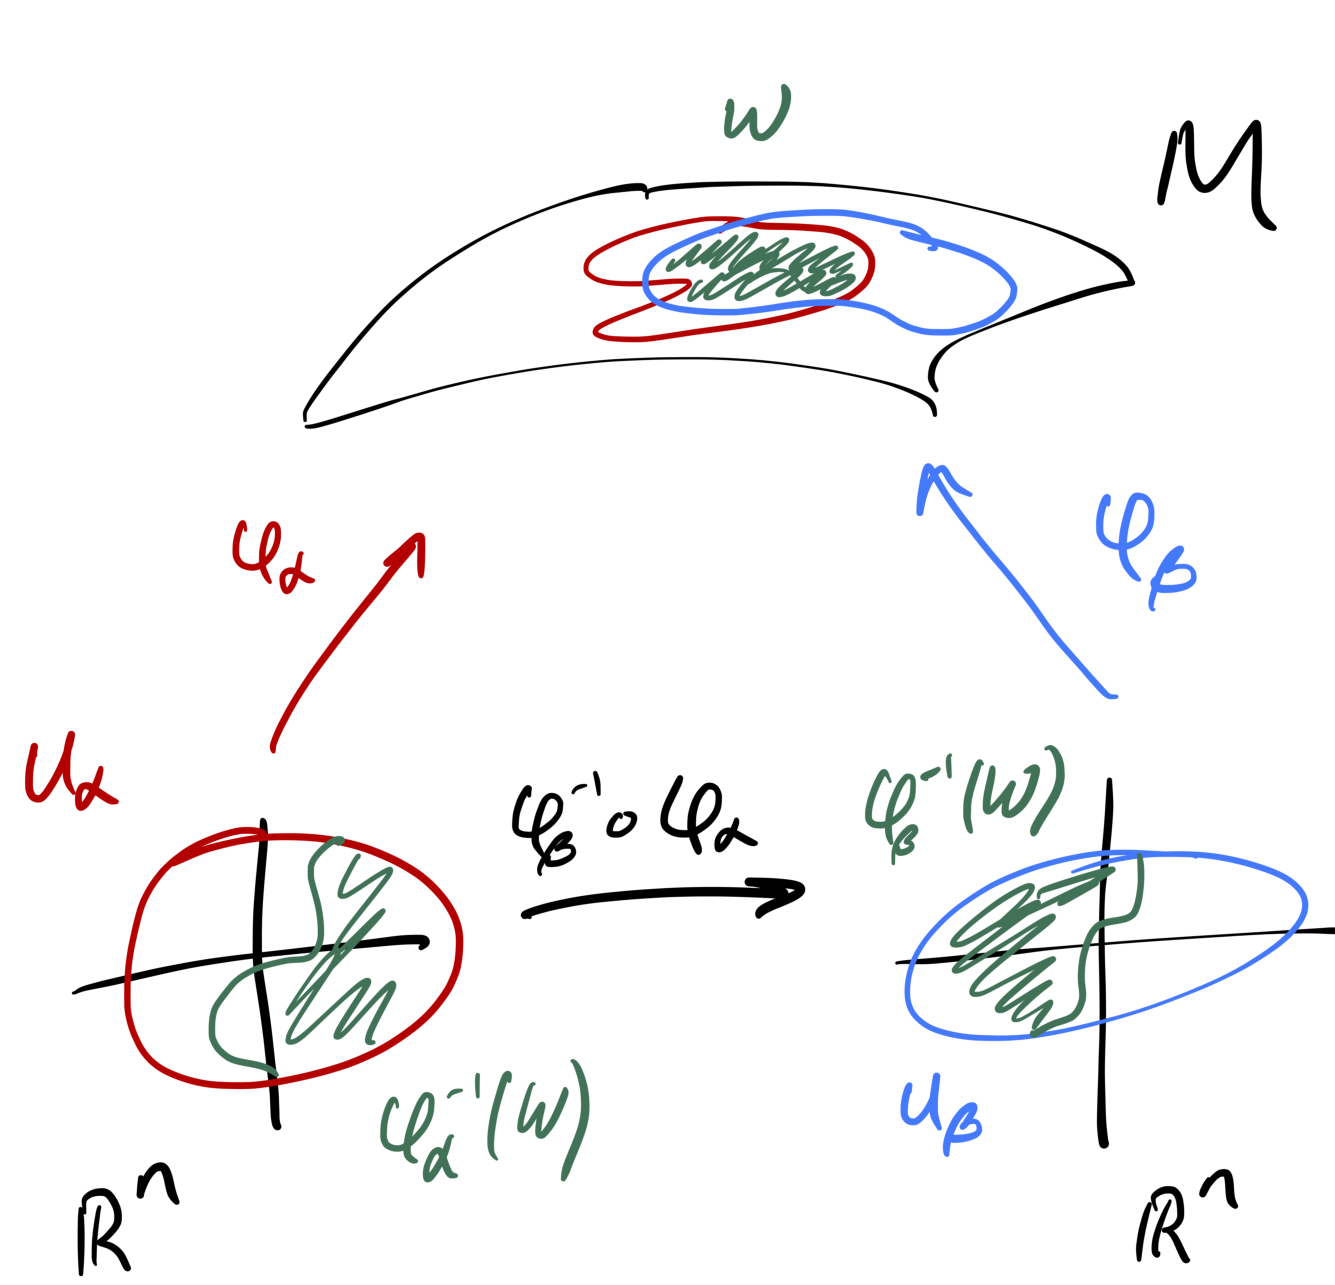
\includegraphics[height=3in]{chart}
	\caption{Transition maps.}
	\label{fig:chart}
\end{figure}

\begin{remark}
	In \ref{it:manifold def overlap} above, ``smooth'' means ``infinitely differentiable'' or, in shorthand, $C^\infty$. What I'm calling \emph{smooth manifolds} are sometimes also called $C^\infty$ \emph{manifolds}. More generally we can talk about $C^\alpha$ manifolds for any integer $\alpha \geq 0$, where we just modify \ref{it:manifold def overlap} to require the maps $\phi_\beta^{-1} \circ \phi_\alpha$ and $\phi_\alpha^{-1} \circ \phi_\beta$ to be $C^\alpha$.\footnote{Recall that a continuous map is $C^\alpha$ if it has $\alpha$ continuous derivatives.} In the special case $\alpha = 0$, this is just a requirement that these maps be continuous, and $C^0$ manifolds are often called \emph{topological manifolds}.
\end{remark}

\begin{example}
	The maximal family containing $(\R^n, \operatorname{id})$ makes $\R^n$ into a smooth manifold.
\end{example}

Of course, most interesting manifolds are not $\R^n$, but the idea of \ref{it:manifold def cover} from \cref{def:manifold} is that you can cover any manifold by a bunch of little open sets (namely, the $\phi_\alpha(U_\alpha)$) that are essentially identical to open sets in $\R^n$ (namely, the $U_\alpha$),\footnote{In topological terms, $U_\alpha$ and $\phi_\alpha(U_\alpha)$ are homeomorphic.} so you can essentially do any local calculation in $\R^n$. It's also very important that the $n$ is always the same here: if $m \neq n$, we're not allowed to have some points with neighborhoods that look like $\R^m$ and some other points whose neighborhoods look like $\R^n$.

If the idea is to use the coordinate charts to transport calculations from the manifold to $\R^n$, then a thing you should be very worried about is that, if a point lies in two different charts, then there are two different ways to do this and they might not be compatible. This is the point of \ref{it:manifold def overlap}: whether you do your calculations in $U_\alpha$ or $U_\beta$, the two are related by a smooth map, so you can easily translate between the two calculations using the change-of-variables formula. Indeed, the usual English-language gloss of \ref{it:manifold def overlap} is that ``transition functions are smooth.''

Finally, \ref{it:manifold def maximal} is a technical condition that in practice is not important. The point of it is simply to ensure uniqueness: if you had a collection of coordinate charts satisfying \ref{it:manifold def cover} and \ref{it:manifold def overlap}, and I took your collection and added some new charts while still satisfying \ref{it:manifold def overlap}, it would be kind of silly to say that you and I were talking about different manifolds. Taking maximal families gives uniqueness since your collection of charts and my collection of charts live in the same maximal family.

% Add discussion that a smooth structure is basically a decision of what should be $C^\infty(M)$, and that, if you don't include \ref{it:manifold def maximal}, then you get ``different'' smooth structures with the same collection of smooth functions.

However, it is certainly possible to have distinct maximal collections on the same space (if there is one that is in some sense standard, then any others are sometimes called ``exotic smooth structures''). At least two Fields Medals have been awarded primarily for finding examples of exotic smooth structures: to John Milnor in 1962 (for finding exotic 7-spheres~\cite{milnorManifoldsHomeomorphic7sphere1956}; it turns out there are exactly 28 distinct smooth structures on $S^7$~\cite{kervaireGroupsHomotopySpheres1963a}) and to Simon Donaldson in 1986 (for finding exotic $\R^4$s~\cite{freedmanTopologyFourdimensionalManifolds1982,donaldsonApplicationGaugeTheory1983,gompfThreeExotic$mathbfR^4$s1983}; it turns out there are uncountably many distinct smooth structures on $\R^4$~\cite{taubesGaugeTheoryAsymptotically1987}). It remains an open problem called the \emph{smooth 4-dimensional Poincaré conjecture} whether there are non-standard differentiable structures on $S^4$.

\begin{remark}
	We often mimic the $\R^n$ notation and indicate the dimension of a manifold $M$ with a superscript; i.e., $M^n$ means that $M$ is an $n$-dimensional manifold, not that we are taking the Cartesian product $M \times M \times \dots \times M$.
\end{remark}

\begin{example}
	$S^n$ the unit sphere in $\R^{n+1}$ is a manifold. Specifically, I claim that the maximal family containing $\{(R^n, \phi_N), (R^n, \phi_S)\}$ makes $S^n$ into an $n$-dimensional manifold, where $\phi_N$ and $\phi_S$ are inverse stereographic projection from the north and south poles, respectively. 
	
	Specifically, with $\vec{x} = (x_1, \dots , x_n) \in \R^n$, define
	\[
		\phi_N(\vec{x}) := \frac{1}{1+\|\vec{x}\|^2}\left(2x_1, \dots , 2x_n, -1+\|\vec{x}\|^2\right)
	\]
	and
	\[
		\phi_S(\vec{x}) := \frac{1}{1+\|\vec{x}\|^2}\left(2x_1, \dots , 2x_n, 1-\|\vec{x}\|^2\right).
	\]
	
	Then $\phi_N$ is the map that sends $\vec{x} \in \R^n$ to the point on the sphere which lies on the line segment connecting $(x_1,\dots , x_n, 0) \in \R^{n+1}$ to the north pole $(0, \dots , 0, 1) \in S^n \subset \R^{n+1}$; see \cref{fig:stereo}. 
	
	\begin{figure}[htbp]
		\centering
			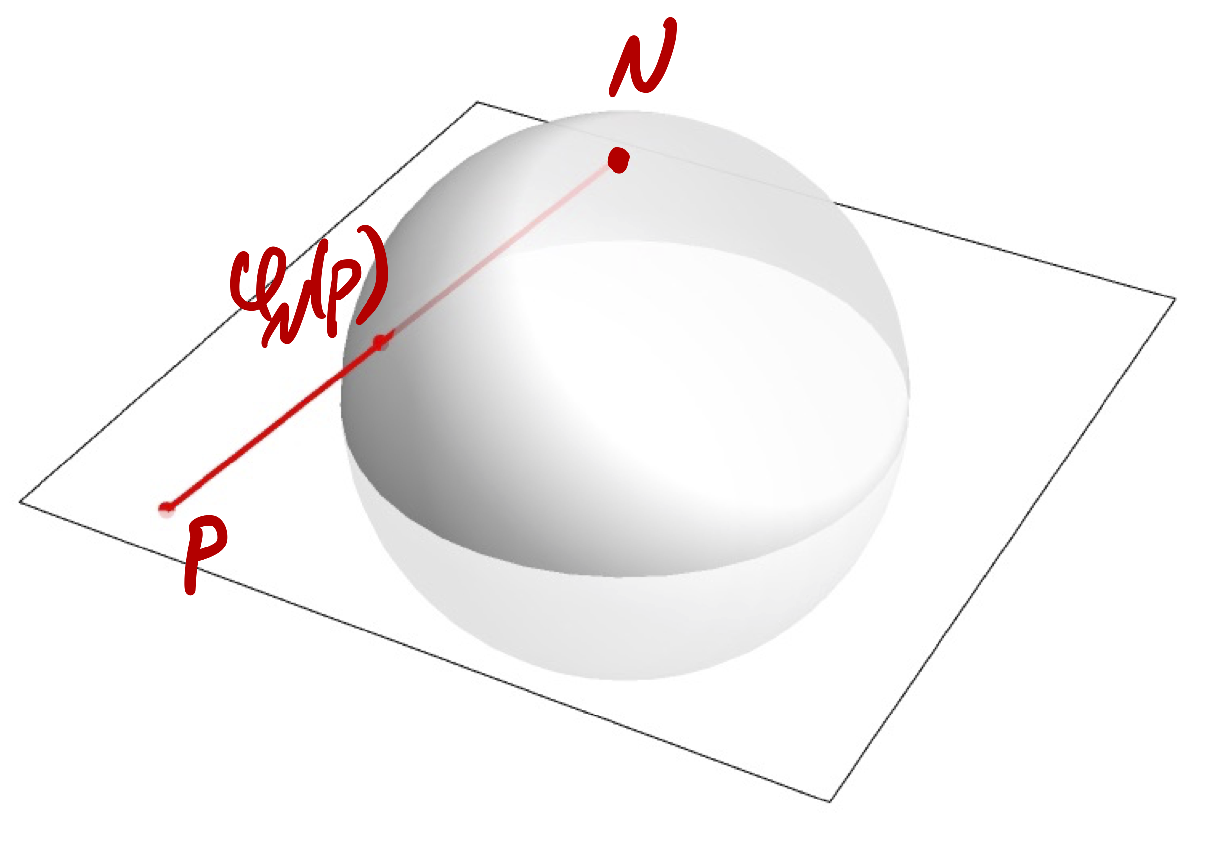
\includegraphics[height=2in]{stereo}
		\caption{Inverse stereographic projection.}
		\label{fig:stereo}
	\end{figure}

To prove the claim, we need to show that \ref{it:manifold def cover} and \ref{it:manifold def overlap} from \cref{def:manifold} are satisfied (\ref{it:manifold def maximal} is automatically satisfied, since we're taking the maximal family containing $\{(\R^n, \phi_N), (\R^n, \phi_S)\}$). 

If we let $N = (0,\dots , 0, 1)$ be the north pole and $S = (0,\dots , 0, -1)$ the south pole, then $\phi_N(\R^n) = S^n \backslash\{N\}$ and $\phi_S(\R^n) = S^n \backslash\{S\}$ and the union is all of $S^n$, so \ref{it:manifold def cover} is satisfied.

For \ref{it:manifold def overlap}, observe that
\[
	W = \phi_N(\R^n) \cap \phi_S(\R^n) = S^n \backslash\{N,S\},
\]
so 
\[
	\phi_N^{-1}(W) = \R^n \backslash\{0\},
\]
which is certainly open, and likewise for $\phi_S^{-1}(W) = \R^n \backslash\{0\}$. So we need to verify that $\phi_N^{-1} \circ \phi_S$ and $\phi_S^{-1} \circ \phi_N$ are smooth as functions on $\R^n \backslash\{0\}$.

The inverse of $\phi_N$ is stereographic projection 
\[
	\phi_N^{-1}(\vec{y}) := \frac{1}{1-y_{n+1}} (y_1, \dots , y_n)
\]
(check this!) so we see that
\[
	(\phi_N^{-1} \circ \phi_S)(\vec{x}) = \frac{1}{\|\vec{x}\|^2}\vec{x}
\]
is reflection through the unit sphere in $\R^n$, which is smooth away from the origin. And similarly for $\phi_S^{-1} \circ \phi_N$.
\end{example}

As already mentioned, the point of manifolds is that they are spaces in which we can do calculus, so we should be able to say what it means for a map between manifolds to be differentiable. Hopefully it's already starting to become clear what the strategy is: we can talk about differentiability at a point, and then both the point in the domain and the point it maps to in the range lie in coordinate charts that are like open sets in Euclidean spaces. So then locally our map just looks like a map between Euclidean spaces, where we already know what it means for a map to be differentiable.

\begin{definition}\label{def:differentiable}
	Let $M^m$ and $N^n$ be manifolds. A continuous map $f\from M \to N$ is \emph{differentiable} at $p \in M$ if, given a coordinate chart $\psi\from V \subseteq \R^n \to N$ containing $f(p)$, there exists a coordinate chart $\phi\from U \subseteq \R^m \to M$ containing $p$ so that $f(\phi(U)) \subseteq \psi(V)$ and 
	\[
		\psi^{-1} \circ f \circ \phi\from U \subseteq \R^m \to \R^n
	\]
	is differentiable at $\phi^{-1}(p)$ (see \cref{fig:differentiable}). The map $f$ is differentiable on an open set in $M$ if it is differentiable at every point in that set.
\end{definition}

\begin{figure}[htbp]
	\centering
		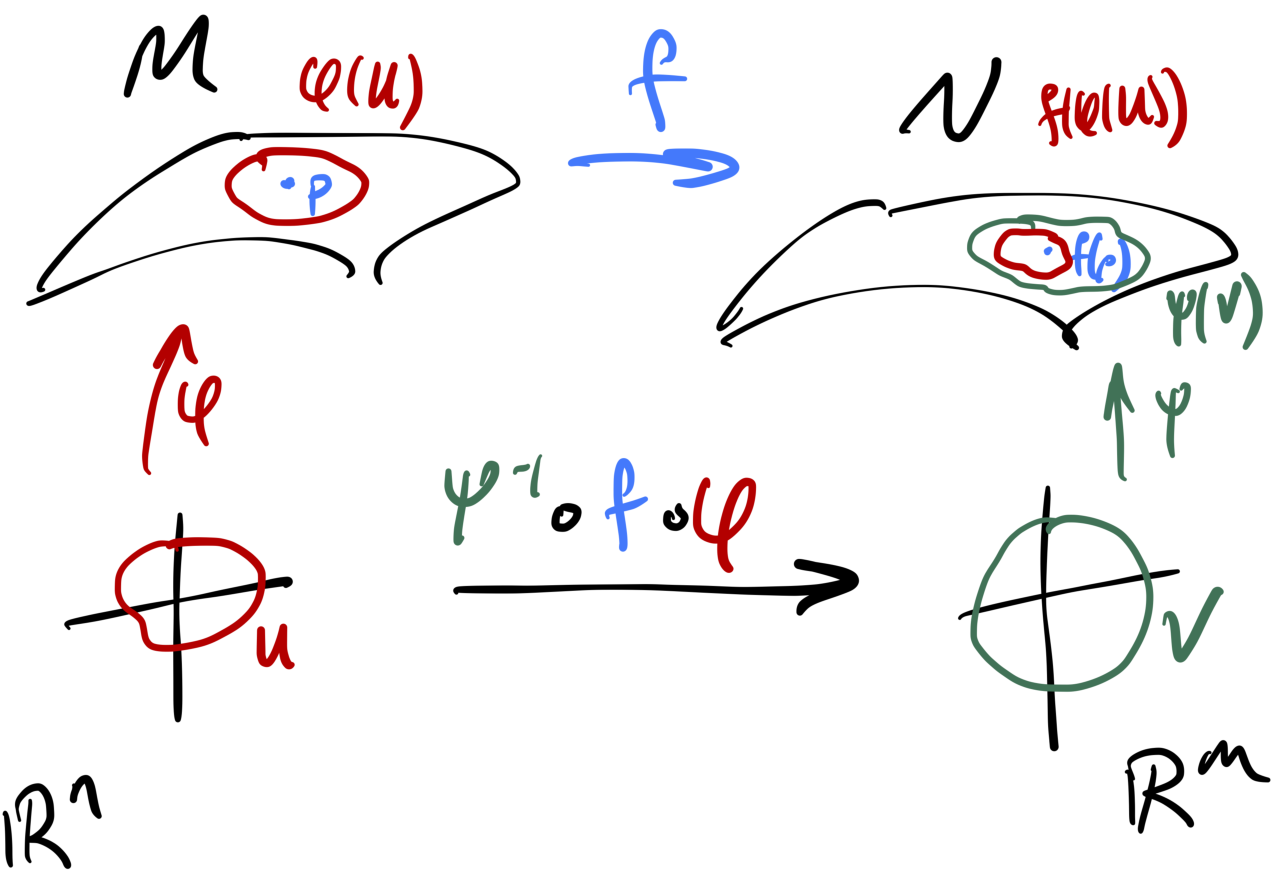
\includegraphics[height=2in]{differentiability}
	\caption{Locally converting a map between manifolds to a map between open sets in Euclidean spaces, where we know what differentiability means.}
	\label{fig:differentiable}
\end{figure}

% Add discussion of why \ref{it:manifold def overlap} implies that if there is \emph{some} coordinate chart in which $\psi^{-1} \circ f \circ \phi$ is smooth, then it will be smooth in \emph{every} coordinate chart.

\begin{example}
	Consider the antipodal map $\alpha \from S^n \to S^n$ given by $\alpha(\vec{y}) = -\vec{y}$. Then, so long as $\vec{y}$ is not the south pole, $\alpha(\vec{y}) = -\vec{y} \in \phi_N(\R^n)$ so we can take $\psi = \phi_N$ and $V = \R^n$. Moreover, $\vec{y} \in \phi_S(\R^n)$ so we can $\phi = \phi_S$ and $U = \R^n$, since $\alpha(\phi_S(\R^n)) = S^n \backslash\{N\} = \phi_N(\R^n)$. Then a straightforward calculation shows that
	\[
		(\phi_N^{-1} \circ \alpha \circ \phi_S)(\vec{x}) = -\vec{x},
	\]
	which is definitely differentiable everywhere (as a map $\R^n \to \R^n$). 
	
	Of course, if $\vec{y} = S$, we can swap the roles of $\phi_N$ and $\phi_S$ in the above, and we conclude that $\alpha$ is differentiable everywhere on $S^n$.
\end{example}

While we've given the definition of a manifold and of a differentiable map in this section, we generally try to use them directly as little as possible. They are hard to handle and fairly unintuitive, so we will quickly be looking for alternative ways of characterizing manifolds and differentiable maps.

% !TEX root = ../dg.tex

\section{Tangent Vectors}

Notice that there's nothing in \cref{def:manifold} that says that a manifold has to live inside some bigger Euclidean space. This is in contrast to a typical undergraduate differential geometry course (like MATH 474 here at CSU), which is typically focused on surfaces in $\R^3$. 

Of course, many manifolds (like spheres) do naturally live in some Euclidean space, and it turns out that the Whitney embedding theorem~\cite{whitneySelfintersectionsSmoothnmanifold1944,whitneySingularitiesSmoothnmanifold1944} guarantees that all manifolds \emph{can} be embedded in some Euclidean space, but this embedding is not necessarily going to be pleasant to work with. If you've encountered them before, it is often much easier to work with projective spaces and Grassmannians \emph{without} embedding them anywhere in particular.

Since our manifolds don't necessarily live inside a Euclidean space, we have to be a bit careful about what a tangent vector at a point is supposed to be. In particular, a tangent vector at a point lives in a different universe than the point itself: the point is a point in the manifold, but the tangent vector does \emph{not} live on the manifold. This is clear even on a sphere in Euclidean space: the tangent vector to a point on the sphere does not live on the sphere! However, in Euclidean space we can kind of cheat and think of both the point and the tangent vector as both living inside the ambient Euclidean space. In general, we can't get away with this.

Now even in Euclidean space you have to be a little careful with this mixing of point and tangent vector: the tangent vector can't be any \emph{arbitrary} vector in the ambient Euclidean space: it has to lie in the \emph{tangent space} at the point, which we usually visualize as some plane which is tangent to the sphere at the point. But if we're not in Euclidean space, things are even worse: if there's supposed to be some subspace which is ``tangent at a point,'' where does it even live? Surely not in the manifold itself, but we're not thinking of the manifold as sitting inside some bigger space, so there's no ``outside'' where it can be.

This is a surprisingly nontrivial issue, requiring us to construct some abstract vector space which doesn't really live anywhere in particular. The construction is fairly non-obvious, and feels like a sneaky trick the first few times you encounter it. This is one of those situations where it seems like you're turning a concept inside-out; at least for me, the first time I encountered the following way of thinking, it made me feel uncomfortable in a similar way to when I first encountered the natural embedding of a vector space into its double dual. I will say that at some point my brain switched from ``this is weird and awkward'' to ``this is obviously the right way to do it'' and I think most differential geometers have had similar experiences, so this is something you can eventually develop intuition for.

% Add something about how ``varying the input a little bit'' can really only mean moving along some curve through the point.

Given that preamble, what's the idea? We're going to work by analogy with a way of thinking about vectors in $\R^n$ that's slightly different from what you may be used to. In words, we'll identify a vector $\vec{v} \in \R^n$ with the operator on differentiable functions which gives the directional derivative (in the direction of $\vec{v}$) of a function. 

That's a little vague, so let's try to characterize a tangent vector $\vec{v}$ to a point $p \in \R^n$ in this way (here I'm using the notation $p$ rather than $\vec{p}$, because I'm just thinking of $p$ as a point in a manifold, not as an element of a vector space). Given $\vec{v}$, I claim we can find some smooth curve $\alpha\from (-\epsilon, \epsilon) \to \R^n$ with $\alpha(0) = p$ and $\alpha'(0) = \vec{v}$; see \cref{fig:tangent vector curve}. In coordinates, if
\[
	\alpha(t) = (x_1(t), \dots , x_n(t)) \quad \text{for } t \in (-\epsilon, \epsilon),
\]
where the coordinate functions $x_i\from (-\epsilon,\epsilon) \to \R$ are themselves smooth, then
\[
	\alpha'(0) = (x_1'(0), \dots , x_n'(0)) = \vec{v}.
\]

\begin{figure}[htbp]
	\centering
		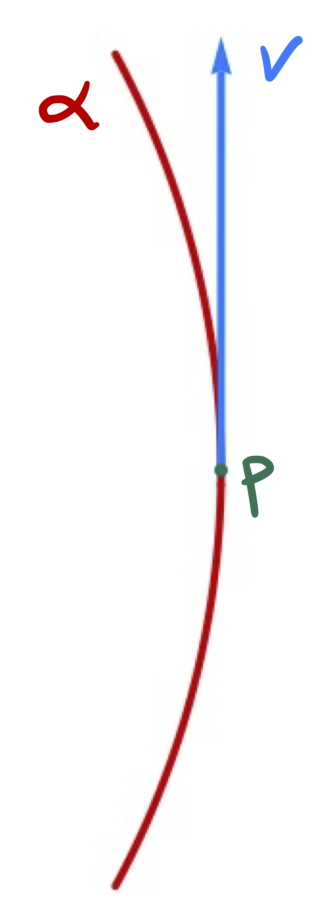
\includegraphics[height=2in]{tangent-vector-curve}
	\caption{A curve through $p$ with velocity $\vec{v}$ at $p$.}
	\label{fig:tangent vector curve}
\end{figure}

(In this specific case, we could take $\alpha(t) = p + t\vec{v}$, but it turns out not to matter which curve satisfying $\alpha(0) = p$ and $\alpha'(0) = \vec{v}$ we take.)

Now, say $f: U \to \R$ is differentiable, where $U \subseteq \R^n$ is some neighborhood of $p$. Then the directional derivative of $f$ at $p$ in the direction of $\vec{v}$ is 
\[
	\left. \frac{d(f \circ \alpha)}{dt} \right|_{t=0} = \sum_{i=1}^n \left.\frac{\partial f}{\partial x_i}\right|_p \left. \frac{d x_i}{dt} \right|_{t=0} = \left(\sum_{i=1}^n x_i'(0) \frac{\partial}{\partial x_i}]\right)f
\]
by the Chain Rule. 

On the right hand side above, we've written the directional derivative as an operator $L = \sum_{i=1}^n x_i'(0) \frac{\partial}{\partial x_i}$ acting on $f$. Moreover, this operator depends uniquely on $\vec{v}$ and is a \emph{linear derivation}, meaning that:
\begin{enumerate}
	\item \label{it:linearity of vector field} $L(f + \lambda g) = L(f) + \lambda L(g)$ for all $f$ and $g$ differentiable in a neighborhood of $p$ and all $\lambda \in \R$;
	\item $L(f g) = f(p) L(g) + g(p) L(f)$ (i.e., the Product Rule).
\end{enumerate}

If it's not clear to you, it's worth looking at the above and convincing yourself that the operator $L$ didn't really depend on the choice of $\alpha$: it really only depends on $p$ and $\vec{v}$ (you may need to go back to the justification from MATH 517 that the directional derivative is well-defined).

The upshot is that, given a point $p$ and a tangent vector $\vec{v}$ at $p$, we get a directional derivative operator $L$. And, conversely, if we know how to compute a directional derivative, we (at least implicitly) know the direction, so this is really a bijective correspondence.

The benefit of thinking in this way is that we can talk about differential operators like $L$ on any manifold; after all, manifolds locally look like $\R^n$ by definition. So, with that long preamble in mind, here's the definition of a tangent vector:

\begin{definition}\label{def:tangent vector}
	Let $M^n$ be a manifold. A smooth function $\alpha\from (-\epsilon, \epsilon) \to M$ is a (smooth) curve in $M$. Suppose $\alpha(0) = p \in M$ and let $\mathcal{D}_p$ be the set of function on $M$ that are differentiable in a neighborhood of $p$. The \emph{tangent vector} to a curve $\alpha$ at $t=0$ is a function $\alpha'(0)\from \mathcal{D}_p \to \R$ given by
	\[
		\alpha'(0)f := \left. \frac{d(f\circ \alpha)}{dt} \right|_{t=0} = (f\circ \alpha)'(0).
	\] 
	A \emph{tangent vector at $p$} is the tangent vector at $t=0$ of some curve $\alpha\from (-\epsilon, \epsilon) \to M$ with $\alpha(0) = p$.
	
	The set of all tangent vectors at $p$ is the \emph{tangent space} to $M$ at $p$, denoted $T_pM$.
\end{definition}

This is a nice coordinate-free way of defining things, but it's not very useful for computations. We usually \emph{do} want to work in coordinates for computations (and certainly for any computations that we want to do on the computer), so let's see what all this means in local coordinates.

Say that $(U,\phi)$ is a coordinate chart containing $p \in M$ so that $\phi(\vec{0}) = p$, that $\alpha \from (-\epsilon , \epsilon) \to M$ is smooth with $\alpha(0) = p$, and that $f$ is a differentiable function in a neighborhood of $p$. Then
\[
	(\phi^{-1} \circ \alpha)(t) = (x_1(t), \dots , x_n(t))
\]
for some smooth functions $x_1 , \dots , x_n\from (-\epsilon, \epsilon) \to \R$. Then
\[
	\alpha'(0) f = \left. \frac{d(f \circ \alpha)}{dt} \right|_{t = 0} = \left. \frac{d}{dt} (f \circ \phi(x_1(t),\dots , x_n(t))) \right|_{t=0} = \left.\sum_{i=1}^n x_i'(0) \frac{\partial f}{\partial x_i}\right|_{\vec{0}} = \left( \left.\sum_{i=1}^n x_i'(0) \frac{\partial }{\partial x_i}\right|_{\vec{0}}\right)f,
\]
where I'm using a very common abuse of notation in the second expression to think of $f$ as being a function on the coordinate chart $U$, and hence a function of coordinates $x_1, \dots , x_n$ (of course, it's really $f \circ \phi$ which is a function of $x_1, \dots , x_n$, as we see in the middle expression).

This all means that we can write the tangent vector $\alpha'(0) \in T_pM$ in local coordinates as
\[
	\alpha'(0) = \sum_{i=1}^n x_i'(0) \left(\frac{\partial}{\partial x_i}\right)_{\vec{0}}.
\]
Since the $x_i'(0)$ are just scalars, what we're doing here is writing $\alpha'(0)$ in terms of the \emph{local coordinate basis} $\left\{\left(\frac{\partial}{\partial x_1}\right)_{\vec{0}}, \dots , \left(\frac{\partial}{\partial x_n}\right)_{\vec{0}}\right\}$ for $T_pM$ associated to the chart $(U,\phi)$.

\begin{remark}
	In practice, we will almost always drop the subscript $\vec{0}$ and just write the basis as $\left\{\frac{\partial}{\partial x_1}, \dots , \frac{\partial}{\partial x_n}\right\}$ and generic tangent vectors as $\sum_{i=1}^n a_i \frac{\partial}{\partial x_i}$.
\end{remark}

\begin{exercise}
	Suppose a point $p \in M$ lies in two different coordinate charts. How are the two different local coordinate bases related?
\end{exercise}

% Add example with tangent vectors on the sphere using stereographic projection.

It's extremely important to keep in mind that, if $p$ and $q$ are distinct points on $M$, then the tangent spaces $T_pM$ and $T_qM$ are \emph{completely different vector spaces} that in principle have nothing to do with each other (they're both vector spaces of the same dimension, and hence abstractly isomorphic, but that's essentially all we can know without more detailed information about the geometry of $M$).

Nonetheless, we often want to talk about all tangent spaces at once, so we smush them together:

\begin{definition}\label{def:tangent bundle}
	The \emph{tangent bundle} of a manifold $M$, denoted $TM$, is the (disjoint) union of tangent spaces
	\[
		TM := \bigsqcup_{p \in M} T_p M.
	\]
	Likewise, if $(T_pM)^\ast$ is the dual of $T_pM$, then the \emph{cotangent bundle} is the union of cotangent spaces
	\[
		T^\ast M := \bigsqcup_{p \in M} (T_pM)^\ast.
	\]
\end{definition}

Notice that there are natural projections $\pi: TM \to M$ and $\widetilde{\pi}: T^\ast M \to M$ which just record the base point; in other words, $\pi$ sends a tangent vector at a point to the point (formally, $TM$ and $T^\ast M$ are \emph{vector bundles}, and this projection is part of their definition).

\begin{theorem}\label{thm:tangent bundles are manifolds}
	If $M$ is an $n$-dimensional manifold, then $TM$ and $T^\ast M$ are $2n$-dimensional manifolds.
\end{theorem}

\begin{exercise}
	Prove \cref{thm:tangent bundles are manifolds}.
\end{exercise}

$T^\ast M$ is, in some sense, the most basic example of a \emph{symplectic manifold}. In physics and dynamical systems language, if $M$ is the \emph{configuration space}\footnote{Meaning it records the positions of particles; for example if we're doing dynamics of $n$ points on the circle, the configuration space is the $n$-torus $S^1 \times \dots \times S^1 = (S^1)^n$.} of a (classical) system, then $T^\ast M$ is \emph{phase space} or \emph{position-momentum space}: this is the natural setting of Hamiltonian mechanics.

\begin{example}
	$T \R^n \cong \R^n \times \R^n \cong \R^{2n}$.
\end{example}

\begin{example}
	$T S^1 \cong S^1 \times \R$, the infinite cylinder.
\end{example}

\begin{example}
	$TS^2$ is a \emph{non-trivial} bundle over $S^2$, meaning that it is \emph{not} homeomorphic to $S^2 \times \R^2$. In particular, one can show that $US^2$, which is the \emph{unit} tangent bundle (the subset of the tangent bundle consisting only of unit tangent vectors) is homeomorphic to $\SO(3) \cong \RP^3$, the real projective space, which is a circle bundle over $S^2$ different from the trivial circle bundle $S^2 \times S^1$. (For those that have taken graduate topology, $\pi_1(S^2 \times S^1) \cong \Z$, whereas $\pi_1(\RP^3) \cong \Z/2\Z$.)
\end{example}
% !TEX root = ../dg.tex

\section{The Differential}

In multivariable calculus, any differentiable map $f \from \R^m \to \R^n$ has a corresponding differential $df$.\footnote{You may have encountered this under the name \emph{Jacobian} rather than \emph{differential}; in the case $n=1$, this is [more or less] the gradient of the function.} While in a multivariable calculus setting we often think of $df$ as a map $\R^m \to \R^n$ as well (meaning it would have the same domain and codomain as $f$), or even more concretely as an $n \times m$ matrix, this is misleading.

In fact, if you were reading the first sentence of the previous paragraph very carefully, you may have noticed that it was not quite correct. Really, I should have said that any differentiable map has a corresponding differential \emph{at a point} $p$. There is no single ``differential'' for a non-linear map: we get different differentials in the neighborhood of each point in the domain.

So more accurately, if $p$ is in the domain of $f$, then we have a differential $df_p$ at $p$. Now, what is the domain of $df_p$? Recall, $df_p$ is supposed to be the best linear approximation of $f$ at $p$, so we're supposed to think of the inputs to $df_p$ as being slight perturbations of $p$. In other words, the domain of $df_p$ is really the tangent space $T_p \R^m$ (which is in a very precise sense the space of \emph{infinitesimal} perturbations of $p$).

Now, $T_p \R^m$ is isomorphic to $\R^m$, but not just in some abstract sense: the tangent bundle $T\R^m$ is trivial, meaning that $T \R^m \cong \R^m \times \R^m$, and a concrete trivialization is given by parallel translating a tangent vector from being based at $p$ to being based at the origin. This is the sense in which we can think of the domain of each $df_p$ as being the ``same'' $\R^m$.

But if $M$ is some more general $m$-dimensional manifold, then, while any tangent space $T_p M$ is still abstractly isomorphic to $\R^m$, the tangent bundle is likely not to be trivial, so we can't make any general identifications of different tangent spaces with the same $\R^m$. So if we want to generalize the notion of differential to manifolds, we need to be careful, even when thinking about functions on $\R^m$, to maintain the distinction between $\R^m$ (thought of an $m$-dimensional manifold) and $T_p \R^m$.

And what about the codomain of $df_p$? Again, we should think more conceptually about what the differential really does. Like all derivatives, the differential tells us something about how the change in an input to a function changes the output of the function. So the inputs to the differential will be tangent vectors at some point in the domain of $f$ (recording an infinitesimal change to the input, or equivalently an initial position [the point] and velocity [the tangent vector] of some path), and the outputs will be tangent vectors at the corresponding point in the range (recording the infinitesimal change in the output). Notice that $T_q \R^n$ is again isomorphic with $\R^n$ by parallel translation.

In other words, given a differentiable map $f \from \R^m \to \R^n$ and a point $p$ in the domain of $f$, the differential of $f$ at $p$ is a map $df_p \from T_p \R^m \to T_{f(p)}\R^n$, where domain and range are usually identified with $\R^m$ and $\R^n$ in a standard way. This, then, is the way of thinking about differentials which generalizes.

\begin{definition}\label{def:differential}
	Suppose $M^m$ and $N^n$ are smooth manifolds and $f \from M \to N$ is smooth. For each $p \in M$, define the \emph{differential} of $f$ at $p$, denoted $df_p\from T_p M \to T_{f(p)}N$, as follows: For any $v \in T_p M$, choose a smooth curve $\alpha \from (-\epsilon, \epsilon) \to M$ such that $\alpha(0) = p$ and $\alpha'(0) = v$. Let $\beta = f \circ \alpha$, which is a smooth curve in $N$. Then
	\[
		df_p(v) := \beta'(0).
	\]
\end{definition}

\begin{lemma}\label{lem:differential is well defined}
	This is a well-defined linear map.
\end{lemma}

\begin{exercise}
	Prove \cref{lem:differential is well defined}.
\end{exercise}

Let's see what this means in local coordinates, which is how we'll actually compute in practice. Suppose $p \in M$ and $(V, \psi)$ is a local coordinate chart on $N$ containing $f(p)$. By \cref{def:differentiable}, there exists some compatible chart $(U, \phi)$ on $M$ containing $p$ so that $f(\phi(U)) \subseteq \psi(V)$. Then the curve $\alpha$ on $M$ (or, really, its restriction to $\phi(U)$) gives a corresponding curve
\[
	(x_1(t), \dots , x_m(t)) = \phi^{-1} \circ \alpha(t)
\]
in $U \subseteq \R^m$, and similarly the curve $\beta$ on $N$ has a corresponding curve
\[
	(y_1(t), \dots , y_n(t)) = \psi^{-1} \circ \beta(t).
\]
See \cref{fig:differential}.

\begin{figure}[htbp]
	\centering
		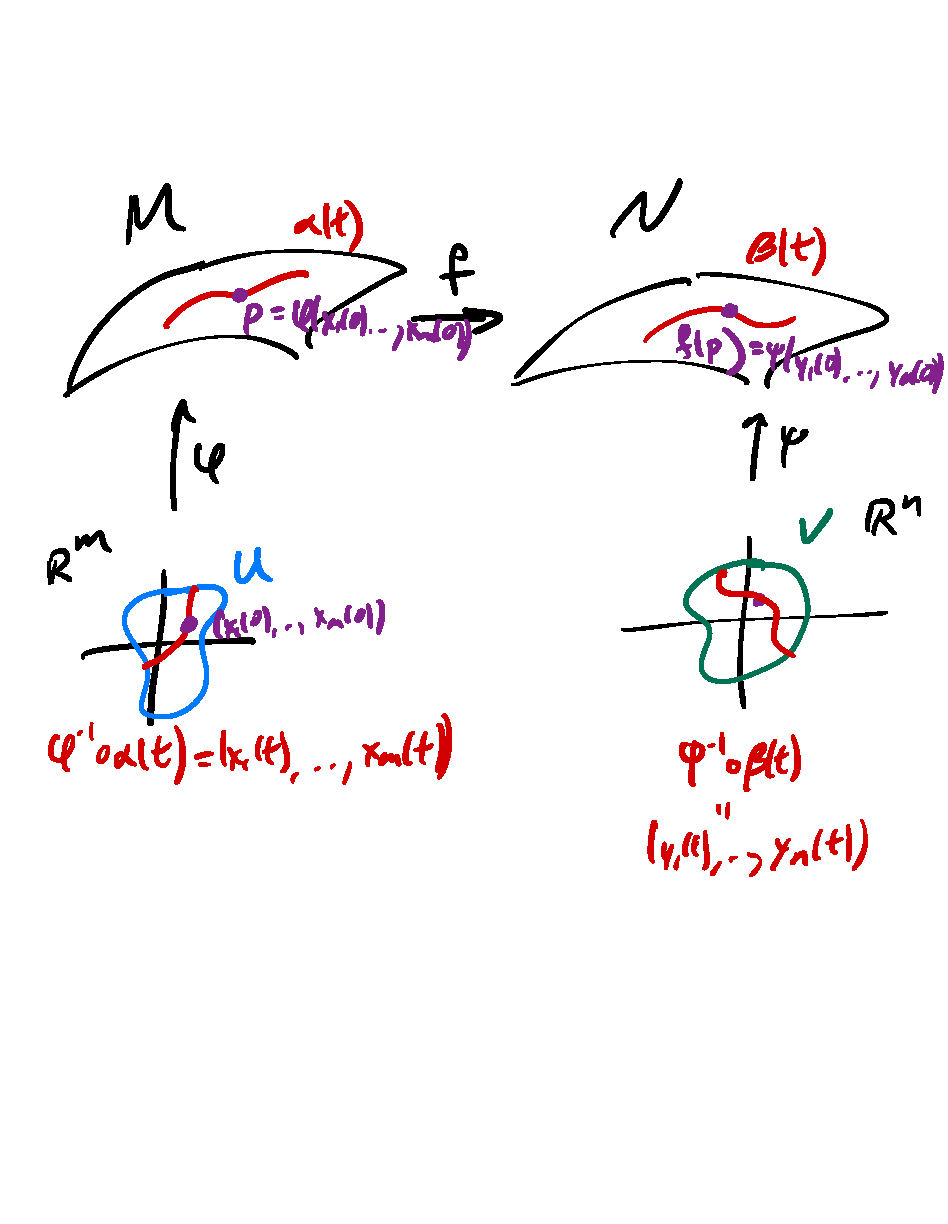
\includegraphics[height=2.5in]{differential}
	\caption{The differential in local coordinates}
	\label{fig:differential}
\end{figure}

Of course,
\[
	\psi^{-1} \circ \beta(t) = \psi^{-1} \circ f \circ \alpha(t) = \psi^{-1} \circ f \circ \phi(x_1(t), \dots , x_m(t)),
\]
so we can think of the $y_i$ as functions of the $x_j$, and the curve in $V$ can be written as
\[
	(y_1(x_1(t),\dots , x_m(t)), \dots , y_n(x_1(t), \dots , x_m(t))).
\]

Working in local coordinates means doing the computation at the level of the map $\psi^{-1} \circ f \circ \phi \from U \subseteq \R^m \to V \subseteq \R^n$, which has a corresponding differential
\[
	d(\psi^{-1} \circ f \circ \phi)_{(x_1(0),\dots , x_m(0))} \from T_{(x_1(0),\dots , x_m(0))} \R^m \to T_{(y_1(0), \dots , y_m(0))} \R^n.
\]
By definition, evaluating this differential on the tangent vector $(x_1'(0), \dots , x_m'(0)) \in T_{(x_1(0),\dots , x_m(0))}\R^m$ gives
\begin{align*}
	\left. \frac{d}{dt} \right|_{t=0} (y_1(x_1(t),\dots , x_m(t)), \dots , y_n(x_1(t),\dots , x_m(t))) & = \left( \sum_{j=1}^m \left.\frac{\partial y_1}{\partial x_j}\right|_{x} \left.\frac{d x_j}{dt} \right|_{t=0}, \dots , \sum_{j=1}^m \left.\frac{\partial y_n}{\partial x_j} \right|_x \left. \frac{d x_j}{dt} \right|_{t=0} \right) \\
	& = \left( \sum_{j=1}^m \left.\frac{\partial y_1}{\partial x_j}\right|_{x} x_j'(0), \dots , \sum_{j=1}^m \left.\frac{\partial y_n}{\partial x_j} \right|_x x_j'(0) \right) \\
	& = \begin{bmatrix} \frac{\partial y_1}{\partial x_1} & \cdots & \frac{\partial y_1}{\partial x_m} \\ \vdots & \ddots & \vdots \\ \frac{\partial y_n}{\partial x_1} & \cdots & \frac{\partial y_n}{\partial x_m} \end{bmatrix} \begin{bmatrix} x_1'(0) \\ \vdots \\ x_m'(0) \end{bmatrix} \\
	& = \begin{bmatrix} \frac{\partial y_i}{\partial x_j} \end{bmatrix}_{i,j} x'(0),
\end{align*}
where $\begin{bmatrix} \frac{\partial y_i}{\partial x_j} \end{bmatrix}_{i,j} $ is the $n \times m$ matrix of partials (i.e., the Jacobian).

So when we work in local coordinates, this is just standard multivariable calculus, as you would hope.

Just to reiterate, the differential (at a point) of a map between manifolds is going to input a tangent vector at a point in the domain and output a tangent vector at a point in the range. As a special case, suppose we have a smooth function on a manifold $M$; that is, a smooth map $f \from M \to \R$. Then, at a point $p \in M$, the differential $df_p \from T_p M \to T_{f(p)}\R$. Now, the tangent bundle to $\R$ is trivial, so we can identify $T_{f(p)}\R$ with $\R$ in a canonical way, and therefore think about $df_p$ as a linear map $T_pM \to \R$.

In other words, by way of this identification of $T_{f(p)} \R$ with $\R$, we can think of $df_p$ as a linear functional on the vector space $T_pM$. Or, in fancier language, $df_p$ is an element of the dual space $\left(T_pM\right)^\ast$. We'll come back to this later when we start talking about differential forms, but this gives a hint of why we might care about cotangent spaces and the cotangent bundle.

Just as in multivariable calculus, when we have a smooth map $f \from M \to N$, we can talk about critical points and critical values, and doing so is often quite important.

\begin{definition}\label{def:critical points}
	Let $f \from M \to N$ be smooth. A point $p \in M$ is a \emph{critical point} of $f$ if $df_p\from T_p M \to T_{f(p)}N$ is not surjective; then $f(p)$ is a \emph{critical value} of $f$. A point $q \in N$ which is not a critical value is a \emph{regular value} of $f$.
\end{definition}

\begin{example}[Cliché Example]
	Consider the function $f$ on the torus depicted in \cref{fig:morse-torus}. In words, $f$ is the height function on this upright torus that just records the $z$-coordinate. I've shown the critical values in red, as well as a couple of regular values in green. Also, back on the torus I've shown the inverse images of the critical and regular values, as well as some tangent vectors to regular points and their images under the differential (in blue and purple), to hopefully convince you the differential really is surjective at these points.
	
	\begin{figure}[htbp]
		\centering
			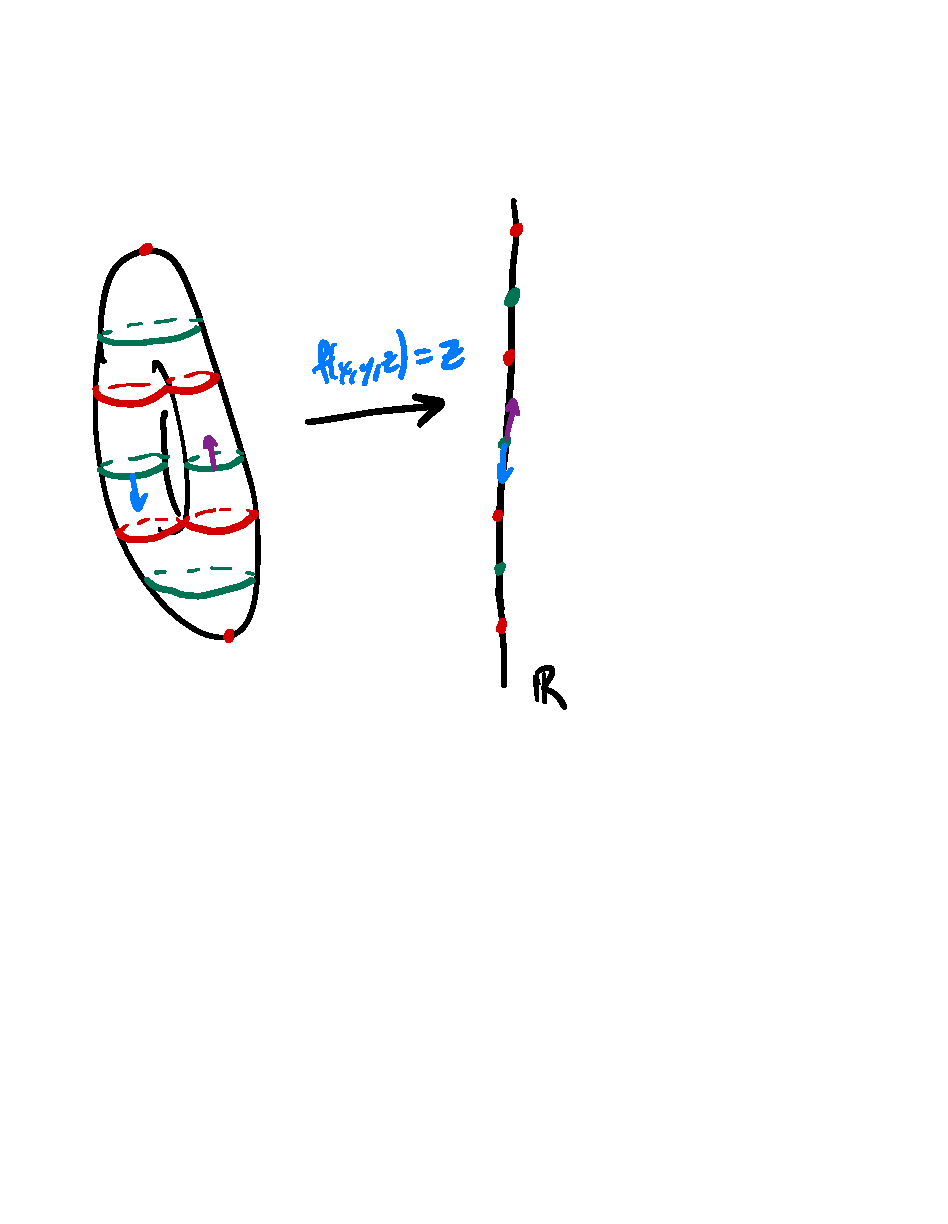
\includegraphics[height=3in]{morse-torus}
		\caption{The height function on a torus.}
		\label{fig:morse-torus}
	\end{figure}
	
	Notice that there are basically three different types of critical points: a minimum, a maximum, and two saddle points. The differential can't possibly be surjective at a (local) minimum: there's no direction you could go which will cause the function to decrease, so the image of the differential has to miss an entire half of its codomain (and therefore, by linearity, everything except the origin). It's somewhat less geometrically clear that the saddle points are critical points, though in this case it's fairly easy to see once you realize the tangent plane to one of the saddle points is horizontal.
	
	A couple of other things to notice about this picture:
	\begin{enumerate}
		\item The inverse images of the two critical points coming from the saddle points contain plenty of regular points: indeed, the differential is surjective at any of the points in the inverse image \emph{except} the saddle point.
		
		\item The level sets of regular values are smooth (collections of) curves, either a single circle or two disjoint circles; in other words, they are smooth (possibly disconnected) 1-dimensional manifolds. The level sets of the critical points are either a single point (the minimum and maximum) or a wedge of two circles (like an $\infty$ symbol). In both cases, the result is not a smooth 1-manifold: a point is a 0-manifold and the wedge of two circles is not locally like a copy of $\R$ near the point where the two circles meet (which of course is exactly the saddle point).
	\end{enumerate}
\end{example}

\begin{remark}
	I call this a cliché example because it is the first picture everybody draws when they talk about Morse theory, which says that the topology of a manifold is in some sense encoded in the critical points of any sufficiently generic function on the manifold. Such functions are called \emph{Morse functions}, and the function in this example is a Morse function. In particular, Morse theory tells you that if you are traversing the manifold ``up'' according to a Morse function, the topology only changes when you pass a critical point. In this example, the topology changes from the empty set to a disk when we pass the minimum, then from a disk to a 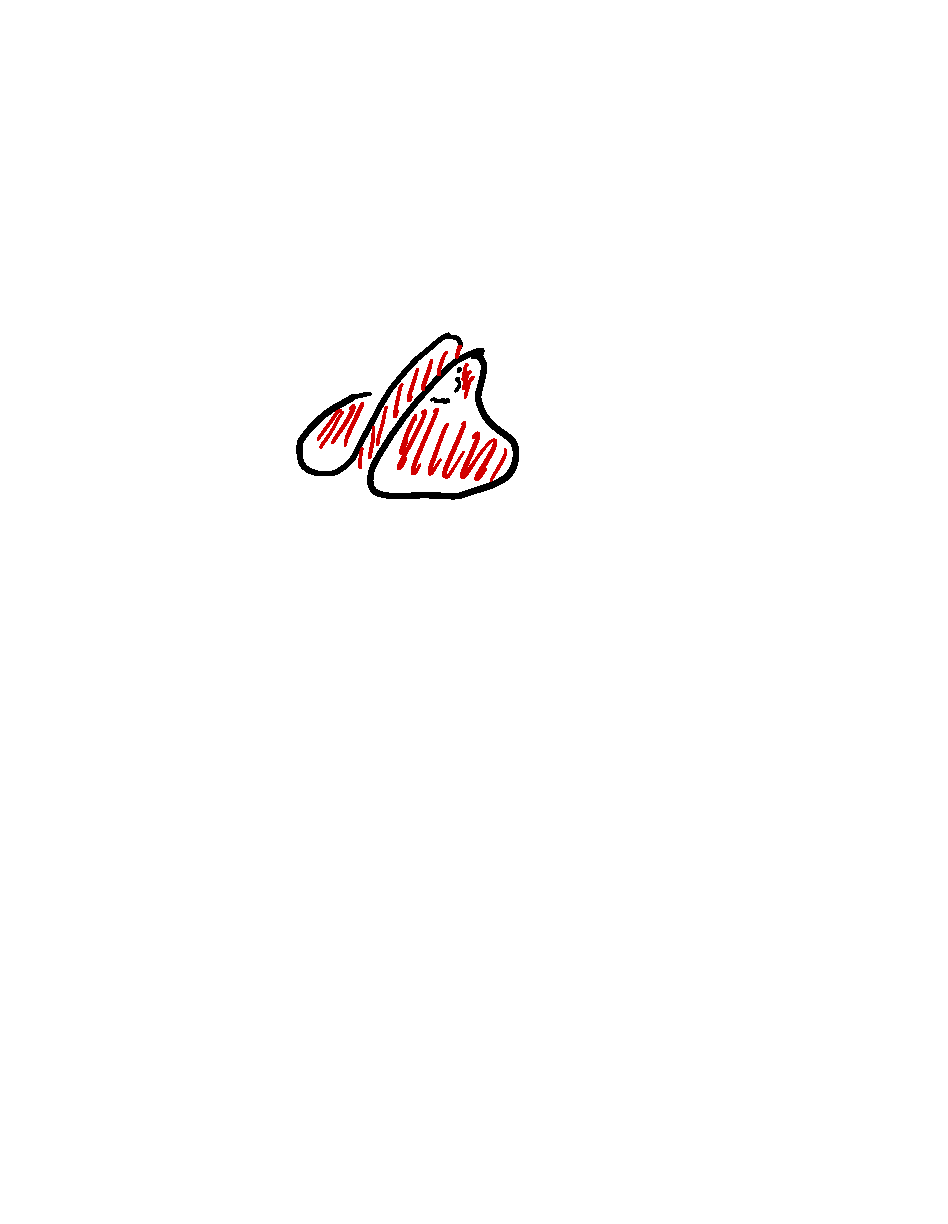
\includegraphics[height=.3in]{handle} (which is homotopic to a circle) when we pass the first saddle point, then to a punctured torus (which is homotopic to a wedge of circles) when we pass the second saddle point, and then finally the puncture is filled in when we pass the maximum. Something analogous happens in general.
\end{remark}

\begin{example}
	Consider the function $f(x,y,z) = z^2$ on the sphere (see \cref{fig:sphere}). Again, I've shown critical values in red and orange and a regular value in green, and the corresponding level sets on the domain, as well as some tangent vectors to regular points and their images under the differential.
	
		\begin{figure}[htbp]
			\centering
				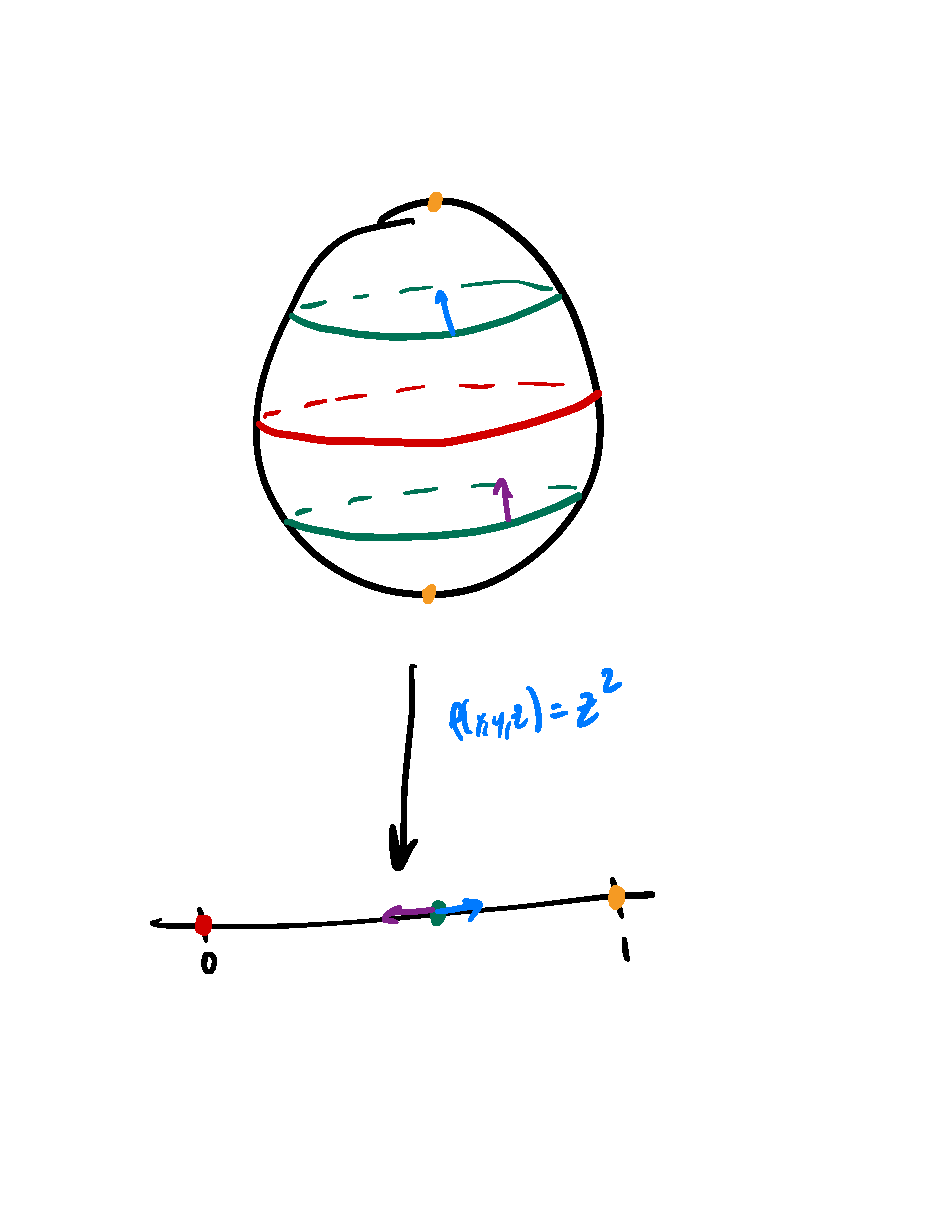
\includegraphics[height=2in]{morse-bott-sphere}
			\caption{A smooth function on the sphere which does not have isolated critical points.}
			\label{fig:sphere}
		\end{figure}
	
	Some new features:
	\begin{enumerate}
		\item The critical points aren't all isolated: the entire equator consists of critical points (which are all global minima).
		
		\item The inverse images of critical values aren't necessarily connected: the north and south poles both map to 1.
	\end{enumerate}
	
	Notice again that the level sets of regular values are (collections of) smooth curves. In this case one critical level set is also a smooth curve, and the other is not a curve at all.
	
	(This is not a Morse function because not all critical points are isolated, but it is a \emph{Morse–Bott function}, which is almost as good.)
	\end{example}
	
	After looking at these examples, hopefully the following theorem suggests itself:
	
	\begin{theorem}[Level Set Theorem]\label{thm:level set theorem}
		If $m \geq n$, $f \from M^m \to N^n$ is smooth, and $q \in N$ is a regular value of $f$, then $f^{-1}(q)$ is a smooth submanifold of $M$ of dimension $m-n$.
	\end{theorem}
	
	This theorem is basically an application of the Inverse Function Theorem, but before we work on proving it, let's look at some more examples.
	
	\begin{example}
		Define $f \from \R^n \to \R$ by $f(x_1,\dots , x_n) = x_1^2 + \dots + x_n^2$. Then
		\[
			df_{(x_1, \dots , x_n)}= \begin{bmatrix} \frac{\partial f}{\partial x_1} & \cdots & \frac{\partial f}{\partial x_n} \end{bmatrix} = \begin{bmatrix} 2x_1 & \cdots & 2x_n \end{bmatrix}
		\]
		only fails to be full rank at the origin, so 0 is the only critical value, and for all $r > 0$ the level set $f^{-1}(r)$ is a smooth manifold of dimension $n-1$. But $f^{-1}(r)$ is nothing but the sphere of radius $\sqrt{r}$, so we've just given an alternative (and somehow conceptually prior) proof that spheres are manifolds.
	\end{example}
	
	\begin{example}[Relevant to frame theory]
		Let $\Mat_{d \times N}(\C)$ be the space of $d \times N$ complex matrices. This is trivially a $2dN$-dimensional manifold, since $\Mat_{d \times N} (\C) \cong \C^{dN}$, which is just a copy of $\R^{2dN}$ if you ignore the complex structure. Now, let $\mathcal{H}(d)$ be the space of $d \times d$ Hermitian matrices (i.e., $d \times d$ complex matrices $A$ so that $A^\ast = A$, where $A^\ast$ is the conjugate transpose of $A$) and define the map $\Phi\from \Mat_{d \times N}(\C) \to \mathcal{H}(d)$ by
		\[
			\Phi(A) = A A^\ast.
		\]
		(In frame theory, we would think of $A \in \Mat_{d \times N}(\C)$ as a frame and $A A^\ast$ as the corresponding frame operator.)
		
		I claim that the identity matrix $I_{d \times d} \in \mathcal{H}(d)$ is a regular value of $\Phi$ (\textbf{Exercise:} Prove this); assuming this, the theorem tells us that $\Phi^{-1}(I_{d \times d})$ is a smooth manifold of dimension
		\[
			2dN - d^2 = d(2N-d).
		\]
		
		(Notice that $A \in \Phi^{-1}(I_{d \times d})$ means that the rows of $A$ are Hermitian orthonormal. Since each row is a vector in $\C^N$, this means that we can think of $\Phi^{-1}(I_{d \times d})$ as the space of all [ordered] $d$-tuples of Hermitian orthonormal vectors in $\C^N$. This space is an example of a \emph{Stiefel manifold}, and usually denoted $\operatorname{St}_d(\C^N)$ or $V_d(\C^N)$. In frame theory, $\Phi^{-1}(I_{d \times d})$ is precisely the space of \emph{Parseval frames}.)
	\end{example}
	
	\begin{example}\label{ex:U(d) manifold}
		Let $N=d$ in the previous example. Then $\Phi^{-1}(I_{d \times d})$ is a smooth manifold of dimension $d^2$ that consists of those $d \times d$ complex matrices $A$ so that $AA^\ast = I_{d \times d}$. But this is precisely the unitary group $\U(d)$! So we've proved that $\U(d)$ is a $d^2$-dimensional manifold for any $d$.
	\end{example}
	
	\begin{remark}
		You can play the same game over $\R$ to show that real Stiefel manifolds and the orthogonal group $\operatorname{O}(d)$ are manifolds.
	\end{remark}

% !TEX root = ../dg.tex

\section{Immersions and Embeddings}

Let's work up to proving \cref{thm:level set theorem}, including defining some more terminology.

\begin{definition}\label{def:immersion and embedding}
	Suppose $f \from M \to N$ is smooth. Then $f$ is an \emph{immersion} if $df_p$ is injective for all $p \in M$ (note that this implies $\dim(M) \leq \dim(N)$). 
	
	If $f$ is also a homeomorphism onto its image (continuous bijection with continuous inverse), then $f$ is an \emph{embedding}. The image of an embedding is a \emph{submanifold}. 
	
	If $f$ is bijective and $f^{-1}$ is smooth, then $f$ is a \emph{diffeomorphism}. $f$ is called a \emph{local diffeomorphism} at $p \in M$ if there exist neighborhoods $U$ of $p$ and $V$ of $f(p)$ so that $f \from U \to V$ is a diffeomorphism.
	
	Finally, we say that $f$ is a \emph{submersion} if $df_p$ is surjective for all $p \in M$.
\end{definition}

\begin{example}\label{ex:cusp}
	Define $\alpha \from \R \to \R^2$ by $\alpha(t) = (t^3, t^2)$ (see \cref{fig:cusp}).
	
	\begin{figure}[htbp]
		\centering
			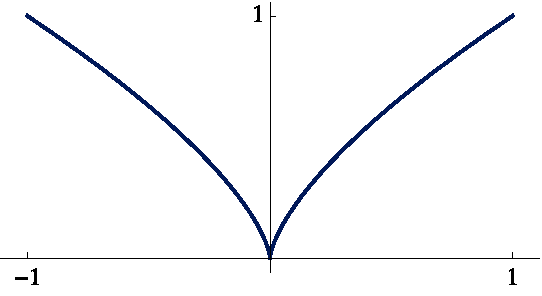
\includegraphics[height=1.5in]{cusp}
		\caption{The image of the map $\alpha$ from \cref{ex:cusp}. The fact that it has a cusp suggests that it will fail to be an immersion, despite being injective and smooth.}
		\label{fig:cusp}
	\end{figure}
	
	This is not an immersion because $d\alpha_0 = \begin{bmatrix} \alpha_1'(0) \\ \alpha_2'(0) \end{bmatrix} = \begin{bmatrix} 0 \\ 0 \end{bmatrix}$ has rank 0. Intuitively, the problem is that the velocity is zero when $t=0$, even though the map overall is continuous and injective.
\end{example}

\begin{example}\label{ex:conic}
	Define $\beta \from \R \to \R^2$ by $\beta(t) = (t^3 - 4t, t^2 - 4)$, which is a deformation of the previous example (see \cref{fig:conic}).
	
	\begin{figure}[htbp]
		\centering
			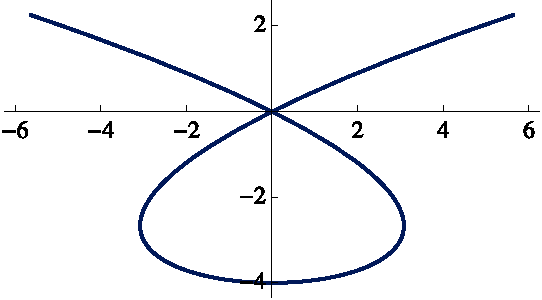
\includegraphics[height=1.5in]{conic}
		\caption{The image of the map $\beta$ from \cref{ex:conic}. This map is an immersion, but not an embedding.}
		\label{fig:conic}
	\end{figure}
	
	Now the differential is given by
	\[
		d\beta_t = \begin{bmatrix} 3t^2 - 4 \\ 2t \end{bmatrix},
	\]
	which is never the zero matrix since the second entry being 0 implies $t=0$, and hence that the first entry is $-4$. Hence, $d\beta_t$ is always rank 1, and hence always injective, so $\beta$ is an immersion.
	
	However, $\beta$ is not an embedding because it is not injective: $\beta(-2) = (0,0) = \beta(2)$, so there is a double point at the origin.
\end{example}

\begin{example}\label{ex:coordinate charts are local diffeomorphisms}
	Suppose $(U,\phi)$ is a local coordinate chart on a manifold $M$ containing a point $p \in M$. Then $\phi \from U \subset \R^n \to M$ is a local diffeomorphism at $\phi^{-1}(p) \in U$. This just follows from the definition of a coordinate chart (\cref{def:manifold}): $\phi$ maps $U$ bijectively onto $\phi(U)$, which is an open neighborhood of $p$, and both $\phi$ and $\phi^{-1}$ are smooth. (To be really pedantic, $(U, \operatorname{id})$ gives a global coordinate chart for the $n$-manifold $U$, and then, following \cref{def:differentiable}, $\phi \from U \to \phi(U)$ is smooth because $\phi^{-1} \circ \phi \circ \operatorname{id} = \operatorname{id}$ is smooth everywhere on $U$. Similarly, $\phi^{-1} \from \phi(U) \to U$ is smooth because $\operatorname{id} \circ \phi^{-1} \circ \phi = \operatorname{id}$ is smooth everywhere on $U$.)
\end{example}

If $f \from M \to N$ is a local diffeomorphism at $p \in M$, then $df_p \from T_pM \to T_{f(p)}N$ is a linear isomorphism (i.e., invertible linear map). Perhaps somewhat surprisingly, the converse is also true. This is the appropriate generalization of the Inverse Function Theorem to the manifold setting, and the proof essentially involves applying the Inverse Function Theorem in local coordinates:

\begin{proposition}\label{prop:local diffeomorphism}
	Suppose $f \from M \to N$ is smooth. If $p \in M$ and $df_p \from T_p M \to T_{f(p)}N$ is an isomorphism, then $f$ is a local diffeomorphism at $p$.
\end{proposition}

\begin{proof}
	We are going to apply the Inverse Function Theorem (\cref{thm:inverse function theorem} below) to $\psi^{-1} \circ f \circ \phi \from \phi(U) \to \psi(V)$, where $(U,\phi)$ and $(V, \psi)$ are the coordinate charts guaranteed to exist by the definition of smoothness (\cref{def:differentiable}).
	
	Notice that, by the Chain Rule,
	\[
		d(\psi^{-1} \circ f \circ \phi)_{\phi^{-1}(p)} = d\psi^{-1}_{f(p)} \circ df_p \circ d\phi_{\phi^{-1}(p)}.
	\]
	But then we already know that $d\phi$ and $d\psi^{-1}$ are isomorphisms (since coordinate charts are local diffeomorphisms [\cref{ex:coordinate charts are local diffeomorphisms}]), so $df_p$ being an isomorphism implies that $d(\psi^{-1} \circ f \circ \phi)_{\phi^{-1}(p)}$ is also an isomorphism.
	
	But then the Inverse Function Theorem implies $\psi^{-1} \circ f \circ \phi$ is a local diffeomorphism at $\phi^{-1}(p)$. Since $\psi$ and $\phi^{-1}$ are local diffeomorphisms (again, \cref{ex:coordinate charts are local diffeomorphisms}) and compositions of local diffeomorphisms are local diffeomorphisms, it follows that
	\[
		\psi \circ (\psi^{-1} \circ f \circ \phi) \circ \phi^{-1} = (\psi \circ \psi^{-1}) \circ f \circ (\phi \circ \phi^{-1}) = f
	\]
	is also a local diffeomorphism.
\end{proof}

Here's a statement of the Inverse Function Theorem in the language of differentials and local diffeomorphisms. It is equivalent to the usual statement you would see in a multivariable calculus or analysis course.

\begin{exercise}
	Convince yourself of the previous sentence.
\end{exercise}

\begin{theorem}[Inverse Function Theorem]\label{thm:inverse function theorem}
	If $F \from U \subseteq \R^n \to \R^n$ is given by $(x_1, \dots , x_n) \mapsto (y_1, \dots , y_n)$, then $dF_p = \begin{bmatrix} \left.\frac{\partial y_i}{\partial x_j}\right|p\end{bmatrix}_{i,j}$ being nonsingular at $p \in U$ implies that $F$ is a local diffeomorphism at $p$.
\end{theorem}

We're now ready to prove the Level Set Theorem (\cref{thm:level set theorem}):

\begin{proof}[Proof of \cref{thm:level set theorem}]
	Recall that, in the statement, we're assuming that $f\from M \to N$ is smooth and that $q \in N$ is a regular value of $f$, and the goal is to show that $f^{-1}(q)$ is a smooth submanifold of $M$ of dimension $m-n$.
	
	Suppose $(U,\phi)$ is a coordinate chart centered at $p \in f^{-1}(q)$\footnote{Meaning that $p = \phi(\vec{0})$.} and $(V, \psi)$ is a chart at $q$. See \cref{fig:level set theorem}. Then define the map
	\[
		g := \psi^{-1} \circ f \circ \phi: U \to \R^n.
	\]
	By assumption,
	\[
		dg_{\vec{0}} = d(\psi^{-1} \circ f \circ \phi)_{\vec{0}} = (d \psi^{-1})_{f(p)} \circ df_p \circ d\phi_{\vec{0}}
	\]
	is surjective since $df_p$ is and the other two terms are isomorphisms.
	
	\begin{figure}[htbp]
		\centering
			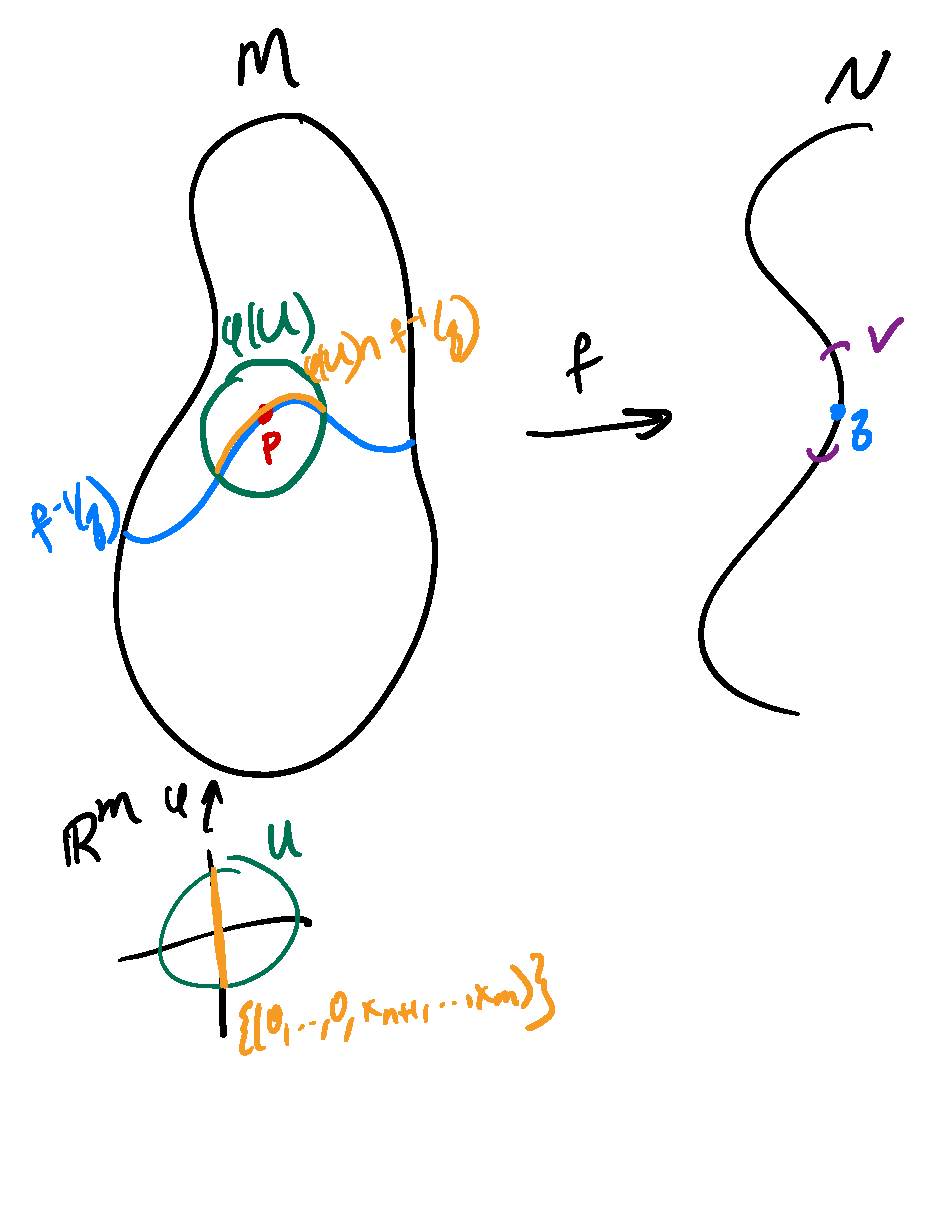
\includegraphics[height=2.5in]{level-set-theorem}
		\caption{A sketch of the key neighborhoods and maps in the proof of \cref{thm:level set theorem}.}
		\label{fig:level set theorem}
	\end{figure}
	
	Hence, after a linear change of coordinates $dg_{\vec{0}}$ can be written as the $n \times m$ block matrix $\begin{bmatrix} I_{n \times n} & 0_{n \times (m-n)} \end{bmatrix}$. Define
	\[
		G(x_1, \dots , x_m) = (g(x_1, \dots , x_n), x_{n+1}, \dots , x_m),
	\]
	which has differential $dG_{\vec{0}} = I_{m \times m}$ in these coordinates. By the Inverse Function Theorem, $G$ is a local diffeomorphism at $\vec{0}$ and by construction $g \circ G^{-1}$ is the standard projection onto the first $n$ coordinates.
	
	So in these coordinates $f^{-1}(1) \cap \phi(U) = \phi(0, \dots , 0, x_{n+1}, \dots , x_m)$, so $x_{n+1} , \dots , x_m$ give local coordinates near $p$ for $f^{-1}(q)$. We can do the same at any other point of $f^{-1}(q)$, so this gives a system of coordinate charts on $f^{-1}(q)$, and the transition maps on overlapping charts are smooth because they are just restrictions (or projections, if you prefer) of the corresponding transition maps for the charts on $M$.
\end{proof}
% % !TEX root = ../dg.tex

\section{Vector Fields}

Now that we have defined tangent vectors and seen how to push them around with differentials, the next natural object to try to define is a vector field. In physical problems, a vector field might be the velocity field of a fluid flow, or an electrical or magnetic field. In both applied and pure problems, we are very often interested in vector fields that arise as the gradients of functions, whether they be Morse functions on an abstract manifold or the energy of conformations in some conformation space. In symplectic geometry we are very interested in Hamiltonian vector fields associated to functions, which are a sort of symplectic gradient. Whereas the gradient is perpendicular to level sets of the function, Hamiltonian vector fields are parallel to level sets, so the function is constant on orbits, which is desirable when the function is an energy function.

So what is a vector field? Intuitively, it's just what you would expect: a choice of tangent vector at each point in the manifold. As with everything in this class, we're mostly interested in \emph{smooth} vector fields, meaning that the tangent vector should in some sense vary smoothly as you move around the manifold.

The preceding sentence hopefully makes sense on an intuitive level, but you should stop and think about how you might try to make it into a rigorous definition. Unless you've already seen the forthcoming definition before, it's probably not so easy.

The problem is that, as alluded to previously, different tangent spaces are not directly comparable. How do you compare $v_1 \in T_{p_1}M$ with $v_2 \in T_{p_2}M$ and, ideally, put them into some difference quotient? 

Since we know how to compare tangent spaces in Euclidean space (by parallel translating), one strategy is to work in local coordinates and require the tangent vectors to form a smooth vector field in each local coordinate chart. But this rather unwieldy, and in any case we want to state definitions without reference to local coordinates if at all possible. Hence the following definition, which encapsulates exactly the idea above in a very concise (though admittedly kind of abstract and hard to visualize) way:

\begin{definition}\label{def:vector field}
	A \emph{vector field} $X$ on a smooth manifold $M$ is a smooth section of the tangent bundle $TM$.
\end{definition}

This requires some unpacking, especially since there's at least one term in this definition which has not been defined yet.

First, recall (\cref{thm:tangent bundles are manifolds}) that $TM$ is a smooth manifold, so it makes sense to talk about smoothness of a map $X\from M \to TM$. So the first part of \cref{def:vector field} is that a vector field is such a smooth map.

This makes sense: such a map takes as input a point in the manifold and outputs a tangent vector. But it would be nonsensical to output a tangent vector at $q$ if the input is $p$: the word ``section'' is how we rule this out.

More precisely, recall that we have a natural projection map $\pi \from TM \to M$ which maps $v \in T_p M$ to the base point $p$. In general, if $E \stackrel{\pi}{\to}B$ is a vector bundle, then a \emph{section} of the bundle is a map $\sigma\from B \to E$ so that $\pi \circ \sigma = \operatorname{id}_B$, the identity map on $B$ (in algebraic terms, $\sigma$ is a right inverse of the projection $\pi$).

So when we say that $X$ is a smooth section of the tangent bundle, we mean that $X \from M \to TM$ is a smooth map satisfying $\pi \circ X = \operatorname{id}_M$. In other words, that $X$ assigns each point in $M$ a tangent vector at that point in a smoothly-varying way. Which is exactly what a (smooth) vector field should be!

\begin{notation}
	We use the notation $\mathfrak{X}(M)$ to denote the $C^{\infty}(M)$-module of vector spaces on $M$.
\end{notation}

\begin{remark}
	\begin{enumerate}
		\item If $\phi \from U \subseteq \R^n \to M$ is a local coordinate chart at $p \in M$, then 
		\[
			X(p) = \sum_{i=1}^n a_i(p) \frac{\partial }{\partial x_i},
		\]
		where each $a_i \from U \to \R$ is smooth and $\left\{\frac{\partial}{\partial x_i}\right\}_i$ is the local coordinate basis of $T_pM$ associated to $(U,\phi)$. Notice that this is exactly the local coordinate definition of a smooth vector field informally formulated above.
		
		\item Since each individual tangent vector is really a directional derivative at a point, a vector field can be interpreted as a differential operator on $M$: it will input a smooth function and output some new smooth function which records the directional derivative at each point in the direction specified by the tangent vector at that point. In other words, we can also interpret a vector field $X$ on a manifold $M$ as a map $C^\infty(M) \to C^\infty(M)$ given by $f \mapsto Xf$. In local coordinates, the function $Xf$ is given by
		\[
			(Xf)(p) = \sum_{i=1}^n a_i(p) \left.\frac{\partial f}{\partial x_i}\right|_p,
		\]
		which is indeed a smooth function.
	\end{enumerate}
\end{remark}

\begin{example}\label{ex:left invariant vector field}
	Consider the unitary group $\U(d)$ and let $I = I_{d \times d}$ be the identity matrix. I claim that a choice of tangent vector at the identity actually determines a vector field on all of $\U(d)$.
	
	To see this, recall that an element of $T_I \U(d)$ is a tangent vector, which is to say, the velocity of a smooth curve $\alpha \from (-\epsilon, \epsilon) \to \U(d)$ with $\alpha(0) = I$. If we think of $\U(d)$ as living inside $\Mat_{d \times d}(\C) \cong \C^{d^2} \cong \R^{2d^2}$, then we can think of any tangent vector $\alpha'(0)$ as a $d \times d$ complex matrix. What restrictions does being tangent to $\U(d)$ place on this matrix?
	
	Notice that, for all $t$, $\alpha(t) \in \U(d)$, which by definition means that $\alpha(t) \alpha(t)^\ast = I$. Since this is the defining equation of $\U(d)$, differentiating at $t=0$ should give precisely the condition for being in $T_I\U(d)$:
	\[
		0 = \left.\frac{d}{dt}\right|_{t=0} I  = \left. \frac{d}{dt}\right|_{t=0} \left(\alpha(t) \alpha(t)^\ast\right) = \alpha'(0) \alpha(0)^\ast + \alpha(0) \alpha'(0)^\ast = \alpha'(0) + \alpha'(0)^\ast
	\]
	since $\alpha(0) = I = \alpha(0)^\ast$ (note that we're also using $(\alpha(t)^\ast)' = \alpha'(t)^\ast$, which is obvious if you choose a basis and write $\alpha(t)$ as a matrix, but kind of annoying to prove in a coordinate-free way).
	
	So we see that $\alpha'(0)^\ast = -\alpha'(0)$. In other words, elements of $T_I \U(d)$ are precisely the skew-Hermitian matrices.
	
	Next, how do we get from a tangent vector at $I$ to a vector field on all of $\U(d)$? Well, we know how to push vector fields around by differentials of maps, so if we had a map $\U(d) \to \U(d)$ sending $I$ to a specified element $U \in \U(d)$, then its differential would send $\Delta \in T_I \U(d)$ to something in $T_U \U(d)$. Of course, there's an obvious map sending $I$ to $U$: the map which left-multiplies elements of $\U(d)$ by $U$. 
	
	In symbols, for $U \in \U(d)$, define the map $L_U \from \U(d) \to \U(d)$ to be left-multiplication by $U$, namely $L_U(A) := UA$. Then certainly
	\[
		(d L_U)_I \from T_I \U(d) \to T_U \U(d)
	\]
	and so, for any $\Delta \in T_I \U(d)$, we get a vector field $X_\Delta \in \mathfrak{X}(\U(d))$ on $\U(d)$ defined by
	\[
		X_\Delta(U) := (d L_U)_I \Delta.
	\]
	We can make this more explicit by finding a formula for $(d L_U)_I$:
	
	\begin{lemma}\label{lem:differential of left multiplication}
		If $U \in \U(d)$ and $\Delta \in T_I \U(d)$, then
		\[
			(d L_U)_I \Delta = U \Delta.
		\]
	\end{lemma}
	
	\begin{exercise}
		Prove \cref{lem:differential of left multiplication}. The key observation here is that matrix multiplication is linear.
	\end{exercise}
	
	Since $(d L_U)_I \from T_I \U(d) \to T_U \U(d)$ is full rank, it's surjective, so $T_U \U(d)$ consists of matrices of the form $U \Delta$ where $\Delta$ is skew-Hermitian.
	
	
	And now it's clear that, for any $\Delta \in T_I \U(d)$, we get the vector field $X_\Delta$ defined by
	\[
		X_\Delta(U) = U\Delta \in T_U \U(d).
	\]
	This is what's called a \emph{left-invariant} vector field on $\U(d)$, since it is invariant under the action of $\U(d)$ on itself by left-multiplication:
	\[
		(d L_U)_V X_\Delta(V) = X_\Delta(UV).
	\]
	
	\begin{exercise}
		Check this.
	\end{exercise}
	
	In fact, one can show that all left-invariant vector fields are of this form, so there is an identification between the collection of left-invariant vector fields on $\U(d)$ and $T_I \U(d)$.
\end{example}

\begin{remark}
	\begin{enumerate}
		\item There was nothing special about $\U(d)$ in \cref{ex:left invariant vector field}: we could have used any group $G$ which was a manifold (such groups are called \emph{Lie groups}; more on them later!) and gotten the same correspondence between the tangent space at the identity and left-invariant vector fields. This is important because these are the two standard ways differential geometers think about \emph{Lie algebras}, and this construction shows that they are equivalent.
		
		\item More generally, the fact that $T_U \U(d)$ consists of matrices of the form $U \Delta$ where $\Delta$ is skew-Hermitian means that \emph{every} vector field $X \in \mathfrak{X}(\U(d))$ can be written as
		\[
			X(U) = U \Delta_U,
		\]
		where the skew-Hermitian matrix $\Delta_U$ depends on $U$. So then a vector field on $\U(d)$ induces a mapping $\U(d) \to T_I \U(d)$ given by $U \mapsto \Delta_U$.
	\end{enumerate}
\end{remark}	
	
	
	\subsection{The matrix exponential} 
	\label{sub:the_matrix_exponential}
	
	This is not directly related to vector fields, but another reason to be interested in $T_I \U(d)$ (or, more generally, the tangent space at the identity of any Lie group) is that it provides local coordinates on almost all of $\U(d)$ by way of the matrix exponential.
	
	
	First of all, if $\Delta \in T_I \U(d)$ (i.e., $\Delta$ is skew-Hermitian), then I claim that $\exp(\Delta) \in \U(d)$, where $\exp$ is the matrix exponential defined by the power series
	\[
		\exp(\Delta) = I + \Delta + \frac{1}{2!} \Delta^2 + \frac{1}{3!}\Delta^3 + \dots.
	\]
	In other words, the claim is that $\exp \from T_I\U(d) \to \U(d)$.
	
	To see that $\exp(\Delta) \in \U(d)$, we need to show that $\exp(\Delta)\exp(\Delta)^\ast = I$, or equivalently ${\exp(\Delta)^\ast = \exp(\Delta)^{-1}}$. Now
	\begin{align*}
		\exp(\Delta)^\ast & = \left( I + \Delta + \frac{1}{2!} \Delta^2 + \frac{1}{3!}\Delta^3 + \dots \right)^\ast \\
		& = I + \Delta^\ast + \frac{1}{2!} \left(\Delta^2\right)^\ast + \frac{1}{3!}\left(\Delta^3\right)^\ast+ \dots \\
		& = I + \Delta^\ast + \frac{1}{2!} \left(\Delta^\ast\right)^2 + \frac{1}{3!}\left(\Delta^\ast\right)^3 + \dots \\
		& = I + \left(-\Delta\right) + \frac{1}{2!} \left(-\Delta\right)^2 + \frac{1}{3!}\left(-\Delta\right)^3+ \dots \\
		& = \exp(-\Delta),
	\end{align*}
and by expanding the product of power series one can show that
\[
	\exp(\Delta)\exp(\Delta)^\ast = \exp(\Delta)\exp(-\Delta) = \exp(\Delta - \Delta) = I.
\]
(It is absolutely essential in the argument for $\exp(\Delta)\exp(-\Delta) = \exp(\Delta - \Delta)$ that $\Delta$ and $-\Delta$ commute. When $A$ and $B$ are matrices with $AB \neq BA$, it is not necessarily true that $\exp(A)\exp(B) = \exp(A+B)$; see the Baker--Campbell--Hausdorff formula in general~\cite[Chapter~5]{hallLieGroupsLie2015}.)

\begin{claim}
	$\exp \from T_I \U(d) \to \U(d)$ is surjective.
\end{claim}

\begin{proof}
	If $U \in \U(d)$, then the eigenvalues of $U$ are all unit complex numbers $e^{i \theta_1}, \dots , e^{i \theta_d}$, so $U$ has the spectral decomposition
	\[
		U = V \Theta V^\ast,
	\]
	where
	\begin{align*}
		\Theta & = \operatorname{diag}\left(e^{i \theta_1}, \dots , e^{i \theta_d}\right) \\
		& = \operatorname{diag}\left(1 + i \theta_1 + \frac{1}{2!} \left(i\theta_1\right)^2 + \dots , \dots , 1 + i \theta_d + \frac{1}{2!} \left(i\theta_d\right)^2 + \dots \right) \\
		& = \exp(\operatorname{diag}(i\theta_1, \dots , i \theta_d)).
	\end{align*}
	(Note that the set of all such $\Theta$ forms a torus; this turns out to be a \emph{maximal torus} inside $\U(d)$).

	But then $H = V \operatorname{diag}(i\theta_1, \dots , i \theta_d)V^\ast$ is skew-Hermitian, and hence in $T_I\U(d)$, and I claim that
	\[
		U = \exp(H).
	\]
	This follows from the more general fact about exponentiating matrix conjugates stated below in \cref{lem:exponentiating conjugates}.

	Just to verify, let's check this on a random example. Here's a random element of $\U(3)$ (generated in \emph{Mathematica} with {\tt RandomVariate[CircularUnitaryMatrixDistribution[3]]}):
	\[
		U = \begin{bmatrix} -0.392089+0.77069 i & -0.175305-0.0691595 i & 0.460085\, -0.0714797 i \\
 -0.359804+0.151554 i & 0.618136\, +0.524479 i & -0.295949-0.32065 i \\
 0.103894\, +0.298465 i & -0.226492+0.505981 i & -0.312325+0.703749 i \end{bmatrix}.
	\]
	Computing the spectral decomposition yields
	\[
		V = \begin{bmatrix} -0.452698+0.477605 i & 0.724632\, +0. i & -0.203482+0.021487 i \\
 0.0746037\, +0.313061 i & 0.0936111\, +0.271501 i & 0.902192\, +0. i \\
 0.680724\, +0. i & 0.346776\, +0.521707 i & -0.249272+0.286437 i \end{bmatrix}
 \]
 and
 \[
 	 \Theta = \begin{bmatrix} e^{2.58364 i} & 0 & 0 \\
 0 & e^{1.68825 i} & 0 \\
 0 & 0 & e^{0.496512 i} \end{bmatrix}.
	\]
	Therefore,
	\[
		H = \begin{bmatrix} 2.0261 i & -0.135698+0.322419 i & -0.228031-0.343709 i \\
 0.135698\, +0.322419 i & 0.810972 i & -0.498786+0.313484 i \\
 0.228031\, -0.343709 i & 0.498786\, +0.313484 i & 1.93134 i \end{bmatrix},
	\]
	and a calculation shows that $\exp(H) = U$, as desired.
\end{proof}

\begin{lemma}\label{lem:exponentiating conjugates}
	Suppose $A,B \in \Mat_{d \times d}(\C)$. Then
	\[
		\exp(ABA^{-1}) = A \exp(B) A^{-1}.
	\]
\end{lemma}

\begin{proof}
	By definition,
	\begin{multline*}
		\exp(ABA^{-1}) = I + ABA^{-1} + \frac{1}{2!} (ABA^{-1})^2 + \dots  = I + ABA^{-1} + \frac{1}{2!} A B^2 A^{-1} + \dots \\
		= A \left(I + B + \frac{1}{2!} B^2 + \dots \right) A^{-1} = A \exp(B)A^{-1}.
	\end{multline*}
\end{proof}

To recap, we have a surjective map $\exp \from T_I \U(d) \to \U(d)$. Moreover, the non-injectivity of $\exp$ is due to the periodicity of the complex exponential: $e^{i \theta} = e^{i(\theta + 2\pi)}$. So $\exp$ maps the neighborhood of the origin in $T_I \U(d)$ consisting of skew-Hermitian matrices with spectral norm $< \pi$ bijectively onto the neighborhood of $I$ in $\U(d)$ consisting of unitary matrices whose eigenvalues all have argument strictly between $-\pi$ and $\pi$; in other words, this only excludes those unitary matrices with $i$ as an eigenvalue, which is some positive codimension subset of $\U(d)$. So then $\exp$ provides a local coordinate chart in the complement of this subset.


	
	



\printbibliography

\end{document}
